% ======================================================================
% sn-article.tex  --  Mathematical Geosciences submission
%   Springer Nature sn-jnl class  (sn-mathphys-ay = author-year refs)
% Title: A Physics-Informed Deep Learning Framework for Solving the
%        2D Shallow Water Equations in Non-Stationary Flood Environments
% Author: Kouao Laurent Kouadio  (ORCID: 0000-0001-7259-7254)
% ======================================================================

%% Math and Physical Sciences Author-Year Reference Style
\documentclass[pdflatex,sn-mathphys-ay]{sn-jnl}

%%---standard packages--------------------------------------------------
\usepackage{graphicx}
\usepackage{amsmath,amssymb,amsfonts}
\usepackage{mathrsfs}            % \mathscr
\usepackage{booktabs}            % \toprule / \midrule / \bottomrule
\usepackage{multirow}
\usepackage[title]{appendix}    % \begin{appendices}
\usepackage{xcolor}              % \textcolor in figure captions
\usepackage{enumerate}
\usepackage{textcomp}
%%----------------------------------------------------------------------

%%---theorem environments (sn-jnl provides thmstyleone/two/three)------
\theoremstyle{thmstyleone}
\newtheorem{theorem}{Theorem}
\newtheorem{lemma}[theorem]{Lemma}
\newtheorem{corollary}[theorem]{Corollary}
\newtheorem{proposition}[theorem]{Proposition}

\theoremstyle{thmstylethree}
\newtheorem{definition}{Definition}

\theoremstyle{thmstyletwo}
\newtheorem{remark}{Remark}
%%----------------------------------------------------------------------

\raggedbottom

% =======================================================================
\begin{document}

\title[Physics-Informed DRN for Non-Stationary Flood Modelling]{%
  A Physics-Informed Deep Learning Framework for Solving the
  2D Shallow Water Equations in Non-Stationary Flood Environments}

\author*[1,2]{\fnm{Kouao Laurent} \sur{Kouadio}%
  \orcid{0000-0001-7259-7254}}\email{etanoyau@gmail.com}

\affil*[1]{\orgdiv{School of Geosciences and Info-Physics},
  \orgname{Central South University},
  \orgaddress{\city{Changsha}, \state{Hunan 410083}, \country{China}}}

\affil[2]{\orgdiv{Hunan Key Laboratory of Nonferrous Resources and
  Geological Hazards Exploration},
  \orgname{Central South University},
  \orgaddress{\city{Changsha}, \state{Hunan 410083}, \country{China}}}

\affil[3]{\orgdiv{UFR des Sciences de la Terre et des Ressources
  Mini\`{e}res},
  \orgname{Universit\'{e} F\'{e}lix Houphou\"{e}t-Boigny},
  \orgaddress{\city{22~BP~582 Abidjan~22}, \country{C\^{o}te d'Ivoire}}}

\abstract{Accurate, physically consistent flood inundation modelling
under climate non-stationarity remains a fundamental challenge for
hazard science in data-sparse environments.  Classical hydrodynamic
solvers that enforce the 2D Shallow Water Equations (SWEs) guarantee
mass and momentum conservation but are computationally prohibitive for
real-time ensemble forecasting at catchment scale.  Purely data-driven
deep-learning surrogates achieve computational efficiency at the cost
of physical consistency, frequently producing paradoxical
predictions---such as water propagation onto elevated terrain---when
confronted with out-of-distribution extreme events.  Here we introduce
the Physically-Aware Deep Reservoir Network (\textsc{PADR-Net}), a
hybrid framework that embeds the SWE PDE residuals as soft constraints
directly into the network's loss function.  We prove rigorously that
(i) the SWE system is strictly hyperbolic for positive water depth;
(ii) the Deep Reservoir Network is a contraction under the Echo State
Property; (iii) the resulting physics-informed optimisation yields a
quantitative error bound $C(\lambda) = O(\lambda^{-1/2})$, ensuring
that the prediction error decays to zero on the SWE solution manifold
as the penalty weight $\lambda \to \infty$.  The framework is validated
on a harmonized archive of 243 flood events (2000--2024) across three
African macro-regions---West Africa (Niger--Benue), East Africa (Nile
headwaters), and Southern Africa (Limpopo--Zambezi)---constituting a
hydroclimatically diverse, data-sparse testbed.  The physics-informed
configuration ($\lambda=1.0$) improved Spearman rank correlation for
flood severity from 0.42 to 0.59 (+41\%) and achieved a mean
leave-one-region-out Spearman of 0.37, demonstrating stable
generalization across contrasting African flood regimes.}

\keywords{Physics-informed neural networks,
          Shallow water equations,
          Deep reservoir computing,
          Flood inundation,
          Non-stationary extremes,
          Africa}

%%\pacs[MSC Classification]{86A05, 68T07, 65M99}

\maketitle

% =======================================================================
\section{Introduction}
\label{sec:intro}

Floods remain among the most damaging and spatially pervasive natural
hazards, affecting populations, infrastructure, agricultural systems,
and regional economies across a wide range of climatic and
geomorphological settings.  Their impacts are increasingly shaped by
the combined effects of climatic non-stationarity, land-use change,
rapid urban expansion, and the continued settlement of flood-prone
terrain.  Satellite observations have shown that human exposure to
flooding is not merely a passive consequence of hazard occurrence but
is actively changing through the redistribution of population and built
assets into areas where inundation has been observed
\citep{Tellman2021}.  At the same time, global projections indicate
that river flood risk is sensitive to both climate forcing and
socio-economic development pathways, with future changes varying
substantially across regions and hydrological regimes
\citep{Hirabayashi2013,Winsemius2016,Alfieri2016}.  These interacting
drivers make flood prediction and impact estimation difficult,
particularly in data-scarce regions where long hydrometric records,
high-resolution topography, and reliable impact observations are often
limited.

A persistent limitation in conventional flood assessment is the
assumption that rainfall extremes can be translated directly into flood
hazard or reported human impact.  Although precipitation provides the
primary atmospheric forcing for many flood events, its relationship
with inundation is strongly mediated by antecedent soil moisture,
catchment storage, river-network routing, floodplain connectivity,
urban drainage, reservoir regulation, and terrain structure.  This
nonlinear disconnect between precipitation anomalies and regional flood
activity has been described through the concept of ``floodiness'',
which emphasizes that flood occurrence and magnitude cannot be
reliably inferred from rainfall statistics alone
\citep{Stephens2015}.  The problem becomes even more complex in
mountainous and high-energy environments, where flood disasters may
arise from cascading processes such as glacial lake outburst floods,
landslides, sediment entrainment, or dam-break-like releases rather
than from local rainfall intensity alone \citep{Sattar2025}.  A
general flood-impact model must therefore represent not only the
meteorological trigger but also the hydrological memory and physical
routing mechanisms that transform rainfall or water release into
spatially distributed inundation.

Physically based hydrodynamic models provide the most direct route for
representing these processes.  Models based on the two-dimensional
shallow-water equations enforce conservation of mass and momentum and
can reproduce flow acceleration, wetting and drying, floodplain
storage, and terrain-controlled propagation.  Efficient inertial and
local-inertial formulations have made large-scale flood simulation more
tractable while retaining the essential structure of shallow-water
dynamics \citep{Bates2010,Almeida2013,Xia2017}.  These developments
have supported continental and global flood hazard modelling, including
high-resolution inundation products and multi-peril frameworks
designed to represent fluvial, pluvial, and coastal flooding
\citep{Sampson2015,Dottori2016,Trigg2016,Wing2019}.  Operational and
pre-operational forecasting systems have also demonstrated the value of
large-scale hydrometeorological modelling for early warning
\citep{Thielen2009,Alfieri2013,Pappenberger2015}.  Nevertheless,
high-resolution hydrodynamic simulation remains computationally
expensive when repeated over many events, ensemble members, climate
scenarios, or uncertainty realizations.  This limitation is especially
restrictive for real-time prediction and for continental-scale impact
analysis in regions where local hydraulic calibration data are sparse.

Machine-learning models offer an attractive complement because they can
learn nonlinear relationships from high-dimensional hydroclimatic,
topographic, and exposure data with far lower computational cost after
training.  Recurrent architectures, particularly long short-term memory
networks, have substantially improved rainfall--runoff prediction and
large-sample hydrological modelling \citep{Hochreiter1997,Kratzert2019}.
Recent work has further shown that deep learning can generalize useful
hydrological information across ungauged or poorly gauged basins when
large and diverse training data are available \citep{Nearing2024}.
However, purely data-driven models remain vulnerable when confronted
with non-stationary extremes, unseen hydrological regimes, or sparse
training examples.  Without physical constraints, they may reproduce
historical correlations while violating basic hydraulic principles,
such as water conservation, terrain-consistent routing, or momentum
balance.  This weakness is particularly problematic for flood-impact
estimation, where the most important events are often rare,
out-of-distribution, and controlled by coupled hazard--exposure
mechanisms.

The challenge is therefore not to choose between physical modelling and
machine learning, but to construct a framework in which the two forms
of information reinforce one another.  A physically guided surrogate
should retain the speed and flexibility of learning-based prediction
while remaining anchored to the governing equations that define
admissible flood states.  In this study, we develop such a framework
through a Physically-Aware Deep Reservoir Network, denoted
\textsc{PADR-Net}.  The model uses a reservoir architecture to capture
nonlinear hydroclimatic memory from sequences of rainfall, antecedent
wetness, river-state indicators, terrain descriptors, and exposure
covariates.  Its predictions are then regularized by residuals derived
from the shallow-water balance, so that the learned trajectories are
encouraged to remain close to the physically admissible solution
manifold.  This formulation is designed to address the central
difficulty of flood-impact prediction: damaging floods emerge from the
interaction between meteorological forcing, catchment memory,
hydrodynamic propagation, and the spatial concentration of people and
assets in flood-prone environments.

The mathematical development of the framework proceeds by linking the
structure of the shallow-water equations to the stability of the
learning model.  The governing system is shown to be strictly
hyperbolic for positive water depth, which establishes the physical
basis for representing propagating flood waves through real-valued
characteristic speeds.  The reservoir state map is then formulated as a
contractive dynamical system under the echo-state condition, ensuring
that the learned state is controlled by the forcing history rather than
by arbitrary initialization.  Finally, the physics-informed objective is
shown to impose a quantitative bound on the distance between the
predicted trajectory and the shallow-water solution manifold, with the
bound decreasing as the physics weight increases.  These results give a
formal interpretation to the proposed regularization: the physical loss
is not only a numerical penalty but a mechanism that constrains the
surrogate model toward mass- and momentum-consistent flood dynamics.

The empirical design follows the same logic.  We first evaluate
\textsc{PADR-Net} under a controlled synthetic flood-event benchmark in
which rainfall forcing, antecedent wetness, terrain routing, exposure,
and impact generation are known.  This benchmark allows us to test
whether the model recovers the intended hierarchy among rainfall,
memory, hydrodynamics, and exposure.  We then apply the framework to a
harmonized archive of 243 African flood events from 2000--2024,
covering contrasting flood-prone regions including the Niger--Benue
system, the Nile headwaters and Sudan--Ethiopia corridor, and the
Limpopo--Zambezi domain.  Africa provides a particularly important
test bed because flood prediction is constrained by heterogeneous
observation networks, strong hydroclimatic seasonality, rapidly
changing exposure, and large regional differences in rainfall regimes
and basin response \citep{Thiemig2015,Bodian2018,Dosio2017,Nikulin2012}.
The experiments are designed to test not only whether the model fits
past events, but whether it transfers across regions and years under
conditions where rainfall-only predictors are expected to fail.

By integrating hydrodynamic constraints, reservoir-based memory, and
ex-ante exposure features, this work advances a flood-impact modelling
framework that is both physically interpretable and computationally
efficient.  The central hypothesis is that robust prediction of flood
burden requires moving beyond precipitation intensity as the dominant
explanatory variable.  Instead, flood impacts must be understood as the
outcome of coupled climate forcing, antecedent catchment state,
terrain-mediated water routing, and human exposure.  The following
sections formalize this framework, describe the synthetic and African
experiments, and evaluate whether physics-aware learning improves
spatial inundation prediction and impact ranking under transfer across
diverse flood regimes; the detailed data provenance, harmonisation
rules, leakage safeguards, and validation partitions are reported in
Appendix~\ref{app:data_experimental_details}.

% =======================================================================
\section{Methodology}
\label{sec:methodology}

The methodology is designed to test whether flood dynamics and
reported impacts can be explained by event-scale rainfall alone, or
whether reliable prediction requires an explicit coupling between
hydrodynamic physics, antecedent hydroclimatic memory, terrain
structure, and pre-event exposure.  Each flood is represented as an
event--region record indexed by $i=1,\ldots,N$, associated with a
regional domain $\Omega_{r_i}\subset\mathbb{R}^{2}$, an event year
$y_i$, and an event time window
\begin{equation}
  \mathcal{T}_{i}
  =
  \{t:s_i\leq t\leq e_i\},
  \label{eq:event_window}
\end{equation}
where $s_i$ and $e_i$ denote the start and end dates of the event.
Events with incomplete dates are retained for descriptive summaries,
but they are excluded from event-window hydroclimatic modelling unless
a physically defensible temporal window can be assigned.  The resulting
event catalogue combines satellite-observed flood information, disaster
impact records, reanalysis hydroclimatic fields, terrain descriptors,
and gridded population and built-up layers.  Satellite flood maps are
used as observational targets and validation data, whereas exposure
features used for prediction are computed only from information
available before the event, so that the realized inundation polygon does
not enter the predictor set.  The corresponding data provenance,
event-window rules, and harmonisation safeguards are detailed in
Appendices~\ref{app:data_sources}--\ref{app:event_harmonisation}.

For each record, the forcing field is constructed from precipitation,
antecedent wetness, temperature, and terrain variables sampled over
$\Omega_{r_i}$.  The antecedent precipitation accumulated over a memory
scale $\tau$ is written as
\begin{equation}
  P^{\mathrm{ant}}_{i,\tau}
  =
  \frac{
  \displaystyle
  \sum_{t=s_i-\tau}^{s_i-1}
  \sum_{g\in\Omega_{r_i}} A_g P_{t,g}
  }{
  \displaystyle
  \sum_{g\in\Omega_{r_i}} A_g
  },
  \qquad
  \tau\in\{7,14,30,60\},
  \label{eq:antecedent_precip}
\end{equation}
where $A_g$ is the area of grid cell $g$ and $P_{t,g}$ is daily
precipitation.  Soil-moisture memory is computed analogously, replacing
$P_{t,g}$ by the corresponding soil-moisture variable.  Where observed
or routed discharge is available, the pre-event river state is
standardized relative to the seasonal climatology,
\begin{equation}
  R^{\mathrm{ant}}_{i,\tau}
  =
  \frac{1}{\tau}
  \sum_{t=s_i-\tau}^{s_i-1}
  \frac{
    Q_{t,h(i)}-\mu_{h(i),m(t)}
  }{
    \sigma_{h(i),m(t)}+\varepsilon
  },
  \label{eq:river_state}
\end{equation}
where $Q_{t,h(i)}$ is discharge at the hydrologically relevant gauge or
routing node $h(i)$, $\mu_{h(i),m(t)}$ and $\sigma_{h(i),m(t)}$ are the
mean and standard deviation for calendar month $m(t)$, and
$\varepsilon>0$ prevents division by zero.  These variables make the
state of the catchment before the event explicit, which is essential
because regional floodiness is often controlled by storage, routing,
and saturation effects rather than by rainfall magnitude alone
\citep{Stephens2015}.

The physical component of the framework is based on the two-dimensional
shallow-water equations, written in conservative form over
$\Omega_{r_i}$ as
\begin{equation}
  \frac{\partial \mathbf{q}}{\partial t}
  +
  \frac{\partial \mathbf{f}}{\partial x}
  +
  \frac{\partial \mathbf{g}}{\partial y}
  =
  \mathbf{R}
  +
  \mathbf{S}_{b}
  +
  \mathbf{S}_{f}.
  \label{eq:swe_main}
\end{equation}
Here $\mathbf{q}$ is the vector of conserved variables, while
$\mathbf{f}$ and $\mathbf{g}$ are the fluxes in the $x$ and $y$
directions:
\begin{equation}
  \mathbf{q}
  =
  \begin{bmatrix}
    h \\ uh \\ vh
  \end{bmatrix},
  \quad
  \mathbf{f}
  =
  \begin{bmatrix}
    uh \\
    u^{2}h+\tfrac{1}{2}g_{0}h^{2} \\
    uvh
  \end{bmatrix},
  \quad
  \mathbf{g}
  =
  \begin{bmatrix}
    vh \\
    uvh \\
    v^{2}h+\tfrac{1}{2}g_{0}h^{2}
  \end{bmatrix},
  \label{eq:swe_fluxes}
\end{equation}
where $h>0$ is water depth, $u$ and $v$ are depth-averaged velocities,
and $g_{0}$ is gravitational acceleration \citep{Bates2010,Liang2010}.
The source terms represent mass exchange, bed slope, and friction:
\begin{equation}
  \mathbf{R}
  =
  \begin{bmatrix}
    P-I-D+Q^{\mathrm{lat}} \\ 0 \\ 0
  \end{bmatrix},
  \quad
  \mathbf{S}_{b}
  =
  \begin{bmatrix}
    0 \\
    -g_{0}h\,\partial b/\partial x \\
    -g_{0}h\,\partial b/\partial y
  \end{bmatrix},
  \quad
  \mathbf{S}_{f}
  =
  \begin{bmatrix}
    0 \\
    -\tau_{bx}/\rho \\
    -\tau_{by}/\rho
  \end{bmatrix}.
  \label{eq:swe_sources}
\end{equation}
In this formulation, $P$ is precipitation, $I$ is infiltration, $D$ is
drainage loss, $Q^{\mathrm{lat}}$ denotes any lateral inflow, $b$ is
bed elevation, and $\rho$ is water density.  The friction stresses are
evaluated using the Manning closure,
\begin{equation}
  \tau_{bx}
  =
  \rho C_f u\sqrt{u^2+v^2},
  \qquad
  \tau_{by}
  =
  \rho C_f v\sqrt{u^2+v^2},
  \qquad
  C_f
  =
  \frac{g_{0}n^2}{h^{1/3}},
  \label{eq:manning}
\end{equation}
where $n$ is the spatially distributed Manning roughness coefficient
\citep{Almeida2013,Xia2017}.  The bed-elevation field $b(x,y)$ is
derived from high-resolution terrain data, with positive elevation
biases from vegetation and built structures corrected where possible
\citep{Farr2007,Hawker2022}.  The equations are written in full
conservative form because this provides a common physical residual for
training; when simplified hydrodynamic products are used for
benchmarking, they are treated as reference simulations rather than as
the governing definition of the physics loss.

The mathematical stability of Eq.~\eqref{eq:swe_main} follows from
the hyperbolic structure of the flux.  Writing
$\mathbf{q}=(h,q_x,q_y)^\top$, with $q_x=uh$ and $q_y=vh$, gives
$u=q_x/h$ and $v=q_y/h$.  Differentiating the $x$-flux with respect to
$\mathbf{q}$ yields
\begin{equation}
  \mathbf{A}
  =
  \frac{\partial\mathbf{f}}{\partial\mathbf{q}}
  =
  \begin{bmatrix}
    0 & 1 & 0 \\
    c^{2}-u^{2} & 2u & 0 \\
    -uv & v & u
  \end{bmatrix},
  \qquad
  c=\sqrt{g_{0}h}.
  \label{eq:jacobian}
\end{equation}
The characteristic polynomial factorizes as
$(\mu-u)\{(\mu-u)^2-c^2\}=0$, so the three wave speeds are
\begin{equation}
  \lambda_1=u-c,
  \qquad
  \lambda_2=u,
  \qquad
  \lambda_3=u+c.
  \label{eq:eigenvalues}
\end{equation}
Since $h>0$ implies $c>0$, the eigenvalues are real and distinct.
Thus the governing system is strictly hyperbolic wherever water depth
is positive.  This property explains why the formulation can represent
surge fronts and rapidly propagating flood waves, while also providing
a physically meaningful residual against which the learning model can
be constrained.

%%%%%%%%%%%%%%%%%%%%%%%%==============================================

To approximate the evolving flood state while retaining the physical
constraints imposed by Eq.~\eqref{eq:swe_main}, we introduce a
physics-informed deep reservoir formulation, denoted \textsc{PADR-Net}.
The model is designed to map a sequence of hydroclimatic and
geomorphic forcings to a physically admissible flood state.  At each
time step $t$, the input vector
$\mathbf{u}_{i,t}\in\mathbb{R}^{N_{\mathrm{in}}}$ contains event
precipitation, antecedent wetness, river-state indicators, terrain
gradient, flow-accumulation descriptors, seasonal variables, and
regional hydroclimatic indicators.  These variables drive a
high-dimensional reservoir state
$\mathbf{x}_{i,t}\in\mathbb{R}^{N_{\mathrm{res}}}$ according to
\begin{equation}
  \mathbf{x}_{i,t}
  =
  \sigma
  \left(
    \mathbf{W}_{\mathrm{in}}\mathbf{u}_{i,t}
    +
    \mathbf{W}_{\mathrm{res}}\mathbf{x}_{i,t-1}
    +
    \mathbf{b}_{\mathrm{res}}
  \right),
  \label{eq:padr_state}
\end{equation}
where $\mathbf{W}_{\mathrm{in}}$ and $\mathbf{W}_{\mathrm{res}}$ are
fixed random matrices, $\mathbf{b}_{\mathrm{res}}$ is a reservoir bias
term, and $\sigma(\cdot)$ is a bounded nonlinear activation function.
Only the output mapping is optimized.  The predicted conservative
hydrodynamic state is
\begin{equation}
  \hat{\mathbf{q}}_{i,t,g}
  =
  \begin{bmatrix}
    \hat{h}_{i,t,g} \\
    \widehat{uh}_{i,t,g} \\
    \widehat{vh}_{i,t,g}
  \end{bmatrix}
  =
  \mathbf{W}_{\mathrm{out}}
  \mathbf{x}_{i,t,g},
  \label{eq:padr_output}
\end{equation}
where $g$ denotes a grid cell, $\hat{h}_{i,t,g}$ is predicted water
depth, and $\widehat{uh}_{i,t,g}$ and $\widehat{vh}_{i,t,g}$ are the
predicted momentum components.  The corresponding velocity components
are recovered as
\begin{equation}
  \hat{u}_{i,t,g}
  =
  \frac{\widehat{uh}_{i,t,g}}
  {\hat{h}_{i,t,g}+\varepsilon_h},
  \qquad
  \hat{v}_{i,t,g}
  =
  \frac{\widehat{vh}_{i,t,g}}
  {\hat{h}_{i,t,g}+\varepsilon_h},
  \label{eq:padr_velocity}
\end{equation}
with $\varepsilon_h>0$ introduced to avoid numerical instability in
nearly dry cells.

The usefulness of the reservoir representation depends on whether the
state is governed by the input history rather than by arbitrary initial
conditions.  This property is obtained by enforcing a contractive
reservoir.  If $L_{\sigma}$ is the Lipschitz constant of the activation
function and
\begin{equation}
  \alpha_{\mathrm{res}}
  =
  L_{\sigma}
  \left\|
    \mathbf{W}_{\mathrm{res}}
  \right\|_{2}
  <1,
  \label{eq:reservoir_contractivity_condition}
\end{equation}
then, for two states $\mathbf{x}_{i,t}$ and $\mathbf{x}'_{i,t}$ driven
by the same input sequence, Eq.~\eqref{eq:padr_state} gives
\begin{equation}
  \left\|
    \mathbf{x}_{i,t}
    -
    \mathbf{x}'_{i,t}
  \right\|_{2}
  \leq
  \alpha_{\mathrm{res}}
  \left\|
    \mathbf{x}_{i,t-1}
    -
    \mathbf{x}'_{i,t-1}
  \right\|_{2}.
  \label{eq:reservoir_one_step}
\end{equation}
Repeated application over $t$ time steps yields
\begin{equation}
  \left\|
    \mathbf{x}_{i,t}
    -
    \mathbf{x}'_{i,t}
  \right\|_{2}
  \leq
  \alpha_{\mathrm{res}}^{t}
  \left\|
    \mathbf{x}_{i,0}
    -
    \mathbf{x}'_{i,0}
  \right\|_{2},
  \label{eq:reservoir_fading_memory}
\end{equation}
which converges to zero as $t$ increases.  Hence, after a sufficiently
long wash-in period, the reservoir state is determined by the forcing
history.  This fading-memory property is important for flood modelling,
because flood response is controlled not only by instantaneous rainfall
but also by accumulated catchment wetness, river routing, and storage
conditions inherited from earlier times.

The predicted state in Eq.~\eqref{eq:padr_output} is constrained by
the shallow-water balance through a residual operator.  Substitution of
$\hat{\mathbf{q}}_{i,t,g}$ into
Eqs.~\eqref{eq:swe_main}--\eqref{eq:swe_sources} gives
\begin{equation}
  \mathcal{F}
  \left(
    \hat{\mathbf{q}}_{i,t,g}
  \right)
  =
  \begin{bmatrix}
    \mathcal{F}^{h}_{i,t,g} \\
    \mathcal{F}^{x}_{i,t,g} \\
    \mathcal{F}^{y}_{i,t,g}
  \end{bmatrix},
  \label{eq:padr_residual_vector}
\end{equation}
where the continuity residual is
\begin{equation}
  \mathcal{F}^{h}_{i,t,g}
  =
  \frac{\partial \hat{h}}{\partial t}
  +
  \frac{\partial (\hat{u}\hat{h})}{\partial x}
  +
  \frac{\partial (\hat{v}\hat{h})}{\partial y}
  -
  \left(
    P-I-D+Q^{\mathrm{lat}}
  \right),
  \label{eq:padr_mass_residual}
\end{equation}
and the two momentum residuals are
\begin{align}
  \mathcal{F}^{x}_{i,t,g}
  &=
  \frac{\partial (\hat{u}\hat{h})}{\partial t}
  +
  \frac{\partial}{\partial x}
  \left(
    \hat{u}^{2}\hat{h}
    +
    \frac{1}{2}g_{0}\hat{h}^{2}
  \right)
  +
  \frac{\partial}{\partial y}
  \left(
    \hat{u}\hat{v}\hat{h}
  \right)
  +
  g_{0}\hat{h}
  \frac{\partial b}{\partial x}
  +
  \frac{\hat{\tau}_{bx}}{\rho},
  \label{eq:padr_xmomentum_residual}
  \\
  \mathcal{F}^{y}_{i,t,g}
  &=
  \frac{\partial (\hat{v}\hat{h})}{\partial t}
  +
  \frac{\partial}{\partial x}
  \left(
    \hat{u}\hat{v}\hat{h}
  \right)
  +
  \frac{\partial}{\partial y}
  \left(
    \hat{v}^{2}\hat{h}
    +
    \frac{1}{2}g_{0}\hat{h}^{2}
  \right)
  +
  g_{0}\hat{h}
  \frac{\partial b}{\partial y}
  +
  \frac{\hat{\tau}_{by}}{\rho}.
  \label{eq:padr_ymomentum_residual}
\end{align}
The predicted friction stresses are computed as
\begin{equation}
  \hat{\tau}_{bx}
  =
  \rho \hat{C}_{f}
  \hat{u}
  \sqrt{\hat{u}^{2}+\hat{v}^{2}},
  \qquad
  \hat{\tau}_{by}
  =
  \rho \hat{C}_{f}
  \hat{v}
  \sqrt{\hat{u}^{2}+\hat{v}^{2}},
  \qquad
  \hat{C}_{f}
  =
  \frac{g_{0}n^{2}}
  {(\hat{h}+\varepsilon_h)^{1/3}}.
  \label{eq:padr_friction}
\end{equation}
In practice, the derivatives in
Eqs.~\eqref{eq:padr_mass_residual}--\eqref{eq:padr_ymomentum_residual}
are evaluated at collocation points using differentiable numerical
operators.  For a generic variable $\phi$, the discrete temporal and
spatial derivatives are written as
\begin{equation}
  \partial_{t}\phi_{i,t,g}
  \approx
  \frac{
    \phi_{i,t+\Delta t,g}
    -
    \phi_{i,t,g}
  }{\Delta t},
  \qquad
  \partial_{x}\phi_{i,t,g}
  \approx
  \frac{
    \phi_{i,t,g^{+}_{x}}
    -
    \phi_{i,t,g^{-}_{x}}
  }{2\Delta x},
  \qquad
  \partial_{y}\phi_{i,t,g}
  \approx
  \frac{
    \phi_{i,t,g^{+}_{y}}
    -
    \phi_{i,t,g^{-}_{y}}
  }{2\Delta y}.
  \label{eq:padr_discrete_derivatives}
\end{equation}
This makes the physics term computable on the same grid used for the
satellite and hydrodynamic validation products.

The learning problem can be written as a regularized
pseudo-posterior.  Let
$\mathcal{D}_{\mathrm{obs}}$ be the set of observed or benchmark flood
states and $\mathcal{D}_{\mathrm{col}}$ the set of collocation points
where the shallow-water residual is evaluated.  The parameter block is
defined as
\begin{equation}
  \Theta
  =
  \left(
    \mathbf{W}_{\mathrm{out}},
    \sigma^{2}_{y},
    \sigma^{2}_{F},
    \eta
  \right),
  \label{eq:padr_parameter_block}
\end{equation}
where $\sigma^{2}_{y}$ is the observational-error variance,
$\sigma^{2}_{F}$ is the physics-residual variance, and $\eta$ controls
the output-weight regularization.  The data model is
\begin{equation}
  \mathbf{y}^{\mathrm{obs}}_{i,t,g}
  =
  \hat{\mathbf{q}}_{i,t,g}
  +
  \boldsymbol{\epsilon}_{i,t,g},
  \qquad
  \boldsymbol{\epsilon}_{i,t,g}
  \sim
  \mathcal{N}
  \left(
    \mathbf{0},
    \sigma^{2}_{y}\mathbf{I}
  \right),
  \label{eq:padr_data_model}
\end{equation}
whereas the physical residual is treated as a zero-centred
pseudo-observation:
\begin{equation}
  \mathbf{0}
  =
  \mathcal{F}
  \left(
    \hat{\mathbf{q}}_{i,t,g}
  \right)
  +
  \boldsymbol{\xi}_{i,t,g},
  \qquad
  \boldsymbol{\xi}_{i,t,g}
  \sim
  \mathcal{N}
  \left(
    \mathbf{0},
    \sigma^{2}_{F}\mathbf{I}
  \right).
  \label{eq:padr_physics_model}
\end{equation}
Combining Eqs.~\eqref{eq:padr_data_model} and
\eqref{eq:padr_physics_model} with a Gaussian prior on
$\mathbf{W}_{\mathrm{out}}$ gives the joint density
\begin{align}
  \pi
  \left(
    \Theta
    \mid
    \mathcal{D}_{\mathrm{obs}},
    \mathcal{D}_{\mathrm{col}}
  \right)
  &\propto
  \left[
    \prod_{(i,t,g)\in\mathcal{D}_{\mathrm{obs}}}
    \mathcal{N}
    \left(
      \mathbf{y}^{\mathrm{obs}}_{i,t,g}
      \mid
      \mathbf{W}_{\mathrm{out}}\mathbf{x}_{i,t,g},
      \sigma^{2}_{y}\mathbf{I}
    \right)
  \right]
  \nonumber \\
  &\quad\times
  \left[
    \prod_{(i,t,g)\in\mathcal{D}_{\mathrm{col}}}
    \mathcal{N}
    \left(
      \mathbf{0}
      \mid
      \mathcal{F}
      \left(
        \mathbf{W}_{\mathrm{out}}\mathbf{x}_{i,t,g}
      \right),
      \sigma^{2}_{F}\mathbf{I}
    \right)
  \right]
  \nonumber \\
  &\quad\times
  \mathcal{N}
  \left(
    \mathrm{vec}
    \left(
      \mathbf{W}_{\mathrm{out}}
    \right)
    \mid
    \mathbf{0},
    \eta^{-1}\mathbf{I}
  \right)
  p
  \left(
    \sigma^{2}_{y}
  \right)
  p
  \left(
    \sigma^{2}_{F}
  \right)
  p(\eta).
  \label{eq:padr_joint_density}
\end{align}
This expression makes explicit the three sources of information used
by the model: observed flood states, hydrodynamic conservation laws,
and parameter regularity.

Taking the negative logarithm of
Eq.~\eqref{eq:padr_joint_density}, discarding constants independent of
$\mathbf{W}_{\mathrm{out}}$, and collecting terms gives
\begin{align}
  \mathcal{J}
  \left(
    \mathbf{W}_{\mathrm{out}}
  \right)
  &=
  \frac{1}{2\sigma^{2}_{y}}
  \sum_{(i,t,g)\in\mathcal{D}_{\mathrm{obs}}}
  \left\|
    \mathbf{y}^{\mathrm{obs}}_{i,t,g}
    -
    \mathbf{W}_{\mathrm{out}}\mathbf{x}_{i,t,g}
  \right\|_{2}^{2}
  \nonumber \\
  &\quad+
  \frac{1}{2\sigma^{2}_{F}}
  \sum_{(i,t,g)\in\mathcal{D}_{\mathrm{col}}}
  \left\|
    \mathcal{F}
    \left(
      \mathbf{W}_{\mathrm{out}}\mathbf{x}_{i,t,g}
    \right)
  \right\|_{2}^{2}
  \nonumber \\
  &\quad+
  \frac{\eta}{2}
  \left\|
    \mathbf{W}_{\mathrm{out}}
  \right\|_{F}^{2}.
  \label{eq:padr_negative_log}
\end{align}
Multiplying Eq.~\eqref{eq:padr_negative_log} by
$2\sigma^{2}_{y}$ gives the equivalent optimization problem
\begin{equation}
  \mathbf{W}^{*}_{\mathrm{out}}
  =
  \arg\min_{\mathbf{W}_{\mathrm{out}}}
  \left\{
  \mathcal{L}_{\mathrm{data}}
  +
  \lambda_{\mathrm{phys}}
  \mathcal{L}_{\mathrm{phys}}
  +
  \omega
  \left\|
    \mathbf{W}_{\mathrm{out}}
  \right\|_{F}^{2}
  \right\},
  \label{eq:padr_map_objective}
\end{equation}
where
\begin{equation}
  \mathcal{L}_{\mathrm{data}}
  =
  \sum_{(i,t,g)\in\mathcal{D}_{\mathrm{obs}}}
  \left\|
    \mathbf{y}^{\mathrm{obs}}_{i,t,g}
    -
    \mathbf{W}_{\mathrm{out}}\mathbf{x}_{i,t,g}
  \right\|_{2}^{2},
  \qquad
  \mathcal{L}_{\mathrm{phys}}
  =
  \sum_{(i,t,g)\in\mathcal{D}_{\mathrm{col}}}
  \left\|
    \mathcal{F}
    \left(
      \mathbf{W}_{\mathrm{out}}\mathbf{x}_{i,t,g}
    \right)
  \right\|_{2}^{2},
  \label{eq:padr_loss_terms}
\end{equation}
and
\begin{equation}
  \lambda_{\mathrm{phys}}
  =
  \frac{\sigma^{2}_{y}}
  {\sigma^{2}_{F}},
  \qquad
  \omega
  =
  \eta\sigma^{2}_{y}.
  \label{eq:padr_weights}
\end{equation}
Thus, the physics weight has a direct interpretation: it is the ratio
between observational uncertainty and residual uncertainty.  When
$\lambda_{\mathrm{phys}}$ is small, the model behaves like a
data-driven reservoir; when $\lambda_{\mathrm{phys}}$ is large,
predictions are strongly constrained to satisfy mass and momentum
balance.

The role of the physics penalty can be clarified by defining the
physically admissible solution set
\begin{equation}
  \mathcal{M}
  =
  \left\{
    \mathbf{q}:
    \mathcal{F}
    \left(
      \mathbf{q}
    \right)
    =
    \mathbf{0}
  \right\}.
  \label{eq:padr_physical_manifold}
\end{equation}
Since $\mathcal{L}_{\mathrm{phys}}$ is a sum of squared residuals, it
is non-negative and vanishes only when the predicted state belongs to
$\mathcal{M}$.  In a neighbourhood of a stable hydrodynamic solution,
the residual controls the distance to this manifold, so that there
exists $\kappa>0$ satisfying
\begin{equation}
  \mathcal{L}_{\mathrm{phys}}
  \left(
    \hat{\mathbf{q}}
  \right)
  \geq
  \kappa
  d
  \left(
    \hat{\mathbf{q}},
    \mathcal{M}
  \right)^{2},
  \qquad
  d
  \left(
    \hat{\mathbf{q}},
    \mathcal{M}
  \right)
  =
  \inf_{\mathbf{q}\in\mathcal{M}}
  \left\|
    \hat{\mathbf{q}}
    -
    \mathbf{q}
  \right\|_{L^{2}}.
  \label{eq:padr_residual_distance}
\end{equation}
Let $\hat{\mathbf{q}}^{*}_{\lambda}$ be the prediction obtained from
Eq.~\eqref{eq:padr_map_objective}, and let
$\mathbf{q}^{\dagger}\in\mathcal{M}$ be any physically admissible
reference state.  Optimality implies
\begin{equation}
  \mathcal{L}_{\mathrm{data}}
  \left(
    \hat{\mathbf{q}}^{*}_{\lambda}
  \right)
  +
  \lambda_{\mathrm{phys}}
  \mathcal{L}_{\mathrm{phys}}
  \left(
    \hat{\mathbf{q}}^{*}_{\lambda}
  \right)
  \leq
  \mathcal{L}_{\mathrm{data}}
  \left(
    \mathbf{q}^{\dagger}
  \right)
  +
  \omega
  \left\|
    \mathbf{W}^{\dagger}_{\mathrm{out}}
  \right\|_{F}^{2}.
  \label{eq:padr_optimality_bound}
\end{equation}
Using Eq.~\eqref{eq:padr_residual_distance} then gives
\begin{equation}
  d
  \left(
    \hat{\mathbf{q}}^{*}_{\lambda},
    \mathcal{M}
  \right)
  \leq
  \left[
  \frac{
    \mathcal{L}_{\mathrm{data}}
    \left(
      \mathbf{q}^{\dagger}
    \right)
    +
    \omega
    \left\|
      \mathbf{W}^{\dagger}_{\mathrm{out}}
    \right\|_{F}^{2}
  }{
    \kappa
    \lambda_{\mathrm{phys}}
  }
  \right]^{1/2}.
  \label{eq:padr_distance_rate}
\end{equation}
Consequently, increasing $\lambda_{\mathrm{phys}}$ decreases the
distance between the learned prediction and the shallow-water solution
manifold at an $O(\lambda_{\mathrm{phys}}^{-1/2})$ rate, provided the
data misfit remains bounded.  This result explains why the proposed
model is expected to generalize better under extreme or spatially
unseen events than a purely empirical rainfall-impact model: the
prediction is not free to exploit spurious correlations if doing so
violates conservation of water mass or momentum.

The predicted hydrodynamic field is finally summarized into
event-level descriptors that can be used in the impact model.  For each
event $i$, the maximum predicted depth, connected inundation area,
duration of wetness, and cumulative water volume are defined as
\begin{align}
  H^{\max}_{i}
  &=
  \max_{t,g}
  \hat{h}_{i,t,g},
  \label{eq:padr_max_depth}
  \\
  A^{\mathrm{wet}}_{i}
  &=
  \sum_{g}
  A_g
  \mathbb{I}
  \left(
    \max_{t}\hat{h}_{i,t,g}
    \geq h_{0}
  \right),
  \label{eq:padr_wet_area}
  \\
  T^{\mathrm{wet}}_{i}
  &=
  \sum_{t,g}
  \Delta t
  \mathbb{I}
  \left(
    \hat{h}_{i,t,g}
    \geq h_{0}
  \right),
  \label{eq:padr_wet_duration}
  \\
  V^{\mathrm{flood}}_{i}
  &=
  \sum_{t,g}
  A_g
  \Delta t
  \hat{h}_{i,t,g}.
  \label{eq:padr_flood_volume}
\end{align}
Here $h_{0}$ is the wet-cell threshold used consistently in the
validation stage.  These descriptors provide a compact bridge between
the physically constrained flood simulation and the subsequent
statistical analysis of reported impacts.

%%%%%%%%%%%%%%%%%%%%%%%%%%%%%%%%%%===================================

Because the paper also evaluates the determinants of reported flood
burden, the hydrodynamic prediction is translated into event-level
features.  To avoid circularity, the exposure support is defined before
the observed inundation is used.  Let $\widetilde{F}_{i}$ denote a
pre-event hazard support derived from modelled return-period flood
zones, low-lying topographic connectivity, river-network buffers, or
forecastable hydrodynamic envelopes.  The observed footprint
$F^{\mathrm{obs}}_{i}$ is used only for validation and never for
constructing predictors.  The ex-ante support construction and the
formal leakage-control rule are provided in
Appendix~\ref{app:leakage_control}.  Population exposure and built-up
exposure are therefore computed as
\begin{equation}
  E^{\mathrm{pop}}_{i}
  =
  \sum_{g\in\widetilde{F}_{i}}
  H_{y_i,g},
  \label{eq:pop_exposure}
\end{equation}
and
\begin{equation}
  E^{\mathrm{built}}_{i}
  =
  \frac{
    \displaystyle
    \sum_{g\in\widetilde{F}_{i}} A_g B_{y_i,g}
  }{
    \displaystyle
    \sum_{g\in\widetilde{F}_{i}} A_g
  },
  \label{eq:built_exposure}
\end{equation}
where $H_{y_i,g}$ is the gridded population in year $y_i$ and
$B_{y_i,g}$ is the built-up fraction.  This distinction separates the
physical extent of possible flooding from the socio-economic
concentration of assets and people within flood-prone terrain
\citep{Tellman2021}.  Additional landscape covariates include mean
slope, elevation range, upstream drainage area, reservoir proximity,
and the fraction of impervious or urbanized land.

For impact modelling, the primary regression target is the
log-transformed affected population,
\begin{equation}
  y^{A}_{i}
  =
  \log_{10}(A_i+1),
  \label{eq:impact_target}
\end{equation}
where $A_i$ is the reported affected population.  High-impact events
are also represented by
\begin{equation}
  z_i
  =
  \mathbb{I}
  \left(
    A_i\geq Q_{\alpha}(A)
  \right),
  \label{eq:impact_indicator}
\end{equation}
where $Q_{\alpha}(A)$ is the empirical $\alpha$-quantile of affected
population.  The explanatory value of rainfall, memory, exposure, and
hydrodynamic information is assessed using nested predictor sets:
\begin{equation}
  \mathbf{x}^{(1)}_{i}
  =
  \mathbf{x}^{R}_{i},
  \qquad
  \mathbf{x}^{(2)}_{i}
  =
  [
    \mathbf{x}^{R}_{i},
    \mathbf{x}^{M}_{i}
  ],
  \qquad
  \mathbf{x}^{(3)}_{i}
  =
  [
    \mathbf{x}^{R}_{i},
    \mathbf{x}^{M}_{i},
    \mathbf{x}^{E}_{i},
    \mathbf{x}^{H}_{i}
  ].
  \label{eq:nested_features}
\end{equation}
Here $\mathbf{x}^{R}_{i}$ contains rainfall-only descriptors,
$\mathbf{x}^{M}_{i}$ contains antecedent hydroclimatic memory,
$\mathbf{x}^{E}_{i}$ contains ex-ante exposure and landscape
covariates, and $\mathbf{x}^{H}_{i}$ contains hydrodynamic quantities
derived from \textsc{PADR-Net}, such as predicted maximum depth,
duration above a wet threshold, connected flooded area, and cumulative
water volume.  The nested structure is important because every richer
model is evaluated on the same validation split as its simpler
counterpart, so any improvement can be attributed to the added
information class rather than to a change in sampling.  The full
feature-construction workflow, including regional percentile
transformations and hydrodynamic summary variables, is documented in
Appendix~\ref{app:feature_construction}.

The statistical baseline is an elastic-net model,
\begin{equation}
  \hat{y}_{i}
  =
  \beta_{0}
  +
  \mathbf{x}_{i}^{\top}\boldsymbol{\beta},
  \label{eq:elastic_prediction}
\end{equation}
with coefficients obtained by minimizing
\begin{equation}
  \mathcal{J}
  =
  \frac{1}{n}
  \sum_{i=1}^{n}
  \left(
    y_i
    -
    \beta_{0}
    -
    \mathbf{x}_{i}^{\top}\boldsymbol{\beta}
  \right)^2
  +
  \lambda_{\mathrm{en}}
  \left[
    \alpha_{\mathrm{en}}
    \|\boldsymbol{\beta}\|_{1}
    +
    \frac{1-\alpha_{\mathrm{en}}}{2}
    \|\boldsymbol{\beta}\|_{2}^{2}
  \right].
  \label{eq:elastic_loss}
\end{equation}
The linear model is supplemented by random forests and gradient-boosted
decision trees to test whether nonlinear interactions between rainfall,
antecedent wetness, terrain, and exposure improve impact ranking.  Deep
learning hydrology studies motivate the comparison between structured
physical constraints and purely data-driven learning, particularly under
spatial transfer and extreme events \citep{Kratzert2019,Nearing2024}.

The empirical evaluation is conducted over three African flood-prone
macro-regions representing contrasting hydroclimatic regimes: the
Niger--Benue system in West Africa, the Nile headwaters and
Sudan--Ethiopia corridor in East Africa, and the Limpopo--Zambezi
domain in Southern Africa.  Together, these regions provide a
data-scarce but hydrologically diverse test bed, including monsoon
floods, long routing-distance river floods, tropical-cyclone-driven
events, and drought--flood transitions; their domain definitions and
event-inventory logic are summarized in
Appendix~\ref{app:study_domains}.  The event archive is divided
chronologically into training, validation, and test periods, so that the
test set contains later events not seen during model fitting.  Spatial
transfer is evaluated by leave-one-region-out validation, while temporal
transfer is evaluated by leave-one-year-out validation, following the
partitioning protocol in Appendix~\ref{app:train_test_partitioning}.
Missing continuous covariates are imputed using training-set medians
only, and binary missingness indicators are appended to the feature
vector to prevent information leakage, as described in
Appendix~\ref{app:missing_uncertainty}.

Spatial flood prediction is assessed using metrics that penalize both
missed inundation and overprediction.  A grid cell is classified as wet
when $\hat{h}\geq h_{0}$, where $h_{0}$ is a fixed shallow-water
threshold.  The Critical Success Index is
\begin{equation}
  \mathrm{CSI}
  =
  \frac{\mathrm{TP}}
  {\mathrm{TP}+\mathrm{FP}+\mathrm{FN}},
  \label{eq:csi}
\end{equation}
where $\mathrm{TP}$, $\mathrm{FP}$, and $\mathrm{FN}$ denote hits,
false alarms, and misses.  The Nash--Sutcliffe Efficiency is computed
for continuous state variables as
\begin{equation}
  \mathrm{NSE}
  =
  1
  -
  \frac{
    \sum_{k}
    (y_{k}-\hat{y}_{k})^{2}
  }{
    \sum_{k}
    (y_{k}-\bar{y})^{2}
  },
  \label{eq:nse}
\end{equation}
and conservation behaviour is summarized by the normalized cumulative
mass error,
\begin{equation}
  \frac{\Delta M}{M_{\mathrm{total}}}
  =
  \frac{
    \left|
    \sum_{t,g}
    \left(
      M^{\mathrm{pred}}_{t,g}
      -
      M^{\mathrm{ref}}_{t,g}
    \right)
    \right|
  }{
    \sum_{t,g}
    M^{\mathrm{ref}}_{t,g}
    +
    \varepsilon
  }.
  \label{eq:mass_error}
\end{equation}
Impact prediction is evaluated using RMSE, MAE, Spearman rank
correlation, and threshold-independent classification scores for
high-impact events.  Uncertainty is quantified by event-level bootstrap
resampling.  For any metric $\mathcal{M}$ and bootstrap replicates
$b=1,\ldots,B$, the reported 95\% interval is
\begin{equation}
  \mathrm{CI}_{95}(\mathcal{M})
  =
  \left[
    Q_{0.025}
    \left(
      \mathcal{M}^{(1)},\ldots,\mathcal{M}^{(B)}
    \right),
    Q_{0.975}
    \left(
      \mathcal{M}^{(1)},\ldots,\mathcal{M}^{(B)}
    \right)
  \right].
  \label{eq:bootstrap_ci}
\end{equation}
Sensitivity experiments perturb the physics weight $\lambda$, the wet
threshold $h_0$, Manning roughness, drainage-loss assumptions, and
reservoir size.  The unconstrained case $\lambda=0$ is retained as the
data-driven baseline, while the optimal physics-informed configuration
uses the value of $\lambda$ that maximizes validation skill without
inflating mass-balance error.  The bootstrap and sensitivity procedures
are specified in Appendix~\ref{app:missing_uncertainty}.  This design
makes the central test explicit: a model that merely learns historical rainfall--impact
associations should fail under spatial or temporal transfer, whereas a
model constrained by shallow-water dynamics and informed by antecedent
memory and ex-ante exposure should remain more stable when confronted
with non-stationary flood environments.

\begin{figure}[t]
  \centering
  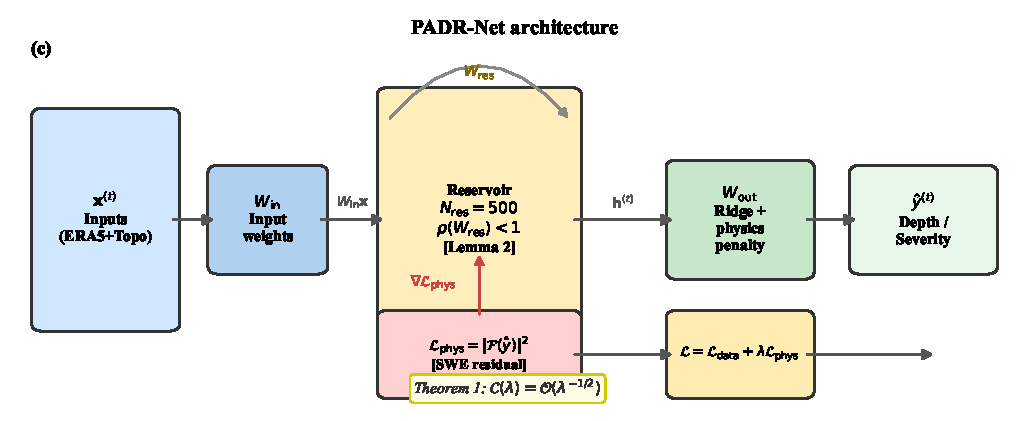
\includegraphics[width=\linewidth]{figures/fig03_architecture}
  \caption{%
    Schematic of the PADR-Net architecture.
    \textbf{(a)}~Input pipeline: per-event ERA5-derived features
    ($\mathbf{x}^R$, $\mathbf{x}^M$, $\mathbf{x}^E$, $\mathbf{x}^H$)
    are mapped through the bimodal Gaussian precipitation
    reconstructor to produce hourly forcing time series
    $P(t)$, $t=1,\ldots,T$.
    \textbf{(b)}~Reservoir layer: the fixed random Echo State Network
    (ESN) with spectral radius $\rho(\mathbf{W}_\mathrm{res})<1$
    (Lemma~\ref{thm:echo_state}) maps $P(t)$ to a high-dimensional
    reservoir state $\mathbf{r}(t)\in\mathbb{R}^N$.
    \textbf{(c)}~Physics-augmented output layer: the augmented ridge
    regression solves for $\mathbf{W}_\mathrm{out}$ by combining the
    SWE analytical depth reference $h^\mathrm{ref}(t)$ (data term)
    and the linearized SWE residual $\mathcal{F}(\hat{h})$ (physics
    term) weighted by $\lambda_\mathrm{phys}$.
    \textbf{(d)}~Calibration and inference: maximum predicted depth
    is converted to a severity proxy through linear calibration on
    the validation split.  Arrow colours indicate information flow:
    blue (data), orange (physics), green (calibration).
  }
  \label{fig:architecture}
\end{figure}


\section{Numerical experiments and experimental setup}
\label{sec:numerical_experiments}

The numerical experiments were designed to evaluate the proposed
physics-informed flood-impact framework under two complementary
conditions.  The first condition uses simulated flood events for which
the forcing, hydrodynamic response, exposure field, and impact
mechanism are fully controlled.  This controlled setting provides a
diagnostic benchmark because the true data-generating process is known;
it therefore allows us to test whether the model can recover the
expected hierarchy among rainfall forcing, antecedent memory,
hydrodynamic response, and exposure.  The second condition uses
observed and remotely sensed flood events from flood-prone African
regions.  This real-data experiment evaluates whether the same
framework remains informative when event timing, reporting quality,
satellite visibility, exposure data, and hydrological observations are
incomplete, heterogeneous, or spatially uneven.  The two experiments
are intentionally linked: the synthetic benchmark establishes the
mathematical and numerical behaviour of the method, whereas the African
application tests its transferability in realistic data-scarce
environments.  Detailed descriptions of the synthetic generator, the
African event inventory, and the spatial-temporal harmonisation
procedures are provided in Appendices~\ref{app:synthetic_generation}
and~\ref{app:data_experimental_details}.

\subsection{Controlled synthetic flood-event benchmark}
\label{subsec:synthetic_benchmark}

For the controlled benchmark, we construct idealized event--region
records over a rectangular spatial domain
$\Omega\subset\mathbb{R}^{2}$ and a discrete time interval
$t=1,\ldots,T$.  The domain is divided into grid cells
$g=1,\ldots,G$, each associated with an area $A_g$, elevation
$b_g$, local slope $s_g$, flow-accumulation index $a_g$, land-cover
class $c_g$, and population density $H_g$.  This synthetic setting is
not intended to reproduce a specific historical flood.  Instead, it is
used to generate controlled flood scenarios in which rainfall intensity,
antecedent catchment wetness, terrain routing, and exposure can be
varied independently.  It therefore provides a transparent way to
verify whether the proposed framework correctly separates
meteorological forcing from hydrological memory and human exposure.
The complete synthetic event-generation rules are reported in
Appendix~\ref{app:synthetic_generation}.

For event $i$, the synthetic rainfall field is generated as
\begin{equation}
  P_{i,t,g}
  =
  P^{0}_{i}
  K_{\ell_i}
  \left(
    g
  \right)
  r_i(t)
  +
  \epsilon^{P}_{i,t,g},
  \label{eq:synthetic_precip}
\end{equation}
where $P^{0}_{i}$ is the event-scale rainfall magnitude,
$K_{\ell_i}(g)$ is a spatial kernel centred on the storm location
$\ell_i$, $r_i(t)$ is the temporal rainfall profile, and
$\epsilon^{P}_{i,t,g}$ is a perturbation term representing unresolved
spatial variability.  The rainfall profile is allowed to vary between
short intense storms and longer multi-day events, so that the synthetic
archive contains both flash-flood-like responses and
basin-storage-dominated responses.

Antecedent wetness is generated as a latent catchment memory state:
\begin{equation}
  M_{i,t,g}
  =
  \rho_M M_{i,t-1,g}
  +
  P_{i,t,g}
  -
  E_{i,t,g},
  \qquad
  0<\rho_M<1,
  \label{eq:synthetic_memory}
\end{equation}
where $E_{i,t,g}$ is potential evapotranspiration and $\rho_M$
controls the persistence of pre-event wetness.  This formulation allows
two events with similar rainfall maxima to produce different flood
responses when their antecedent states differ.

The synthetic flood response is obtained by routing the generated
forcing through the same hydrodynamic operator used in the methodology.
The reference state
$\mathbf{q}^{\mathrm{ref}}_{i,t,g}
=(h^{\mathrm{ref}}_{i,t,g},
u^{\mathrm{ref}}_{i,t,g}h^{\mathrm{ref}}_{i,t,g},
v^{\mathrm{ref}}_{i,t,g}h^{\mathrm{ref}}_{i,t,g})^{\top}$
is computed from the shallow-water balance,
\begin{equation}
  \frac{\partial \mathbf{q}^{\mathrm{ref}}}{\partial t}
  +
  \frac{\partial \mathbf{f}^{\mathrm{ref}}}{\partial x}
  +
  \frac{\partial \mathbf{g}^{\mathrm{ref}}}{\partial y}
  =
  \mathbf{R}^{\mathrm{ref}}
  +
  \mathbf{S}^{\mathrm{ref}}_{b}
  +
  \mathbf{S}^{\mathrm{ref}}_{f},
  \label{eq:synthetic_reference_swe}
\end{equation}
using the terrain, roughness, infiltration, and drainage parameters
assigned to the synthetic domain.  From this reference state we derive
maximum depth, wet duration, connected wet area, and flood volume:
\begin{align}
  H^{\max}_{i}
  &=
  \max_{t,g}
  h^{\mathrm{ref}}_{i,t,g},
  \label{eq:synthetic_hmax}
  \\
  A^{\mathrm{wet}}_{i}
  &=
  \sum_{g=1}^{G}
  A_g
  \mathbb{I}
  \left(
    \max_t h^{\mathrm{ref}}_{i,t,g}\geq h_0
  \right),
  \label{eq:synthetic_awet}
  \\
  V^{\mathrm{flood}}_{i}
  &=
  \sum_{t=1}^{T}
  \sum_{g=1}^{G}
  A_g\Delta t
  h^{\mathrm{ref}}_{i,t,g}.
  \label{eq:synthetic_volume}
\end{align}
Here $h_0$ is the wet-cell threshold used consistently in the spatial
validation.  The reference inundation footprint is used only to create
validation targets.  Predictive exposure features are instead computed
from pre-event hazard supports, denoted $\widetilde{F}_{i}$, generated
from return-period flood zones, low-lying topographic connectivity,
and river-buffer masks.  This prevents circularity because the realized
flood footprint is never used as a predictor.

The synthetic impact outcome is generated from a controlled
multi-evidence mechanism.  Let $\mathbf{x}^{R}_{i}$ denote
rainfall-only features, $\mathbf{x}^{M}_{i}$ antecedent memory
features, $\mathbf{x}^{H}_{i}$ hydrodynamic features, and
$\mathbf{x}^{E}_{i}$ ex-ante exposure features.  The affected
population is generated as
\begin{equation}
  y^{A}_{i}
  =
  \log_{10}
  \left(
    A_i+1
  \right)
  =
  \beta_0
  +
  \boldsymbol{\beta}^{\top}_{R}
  \mathbf{x}^{R}_{i}
  +
  \boldsymbol{\beta}^{\top}_{M}
  \mathbf{x}^{M}_{i}
  +
  \boldsymbol{\beta}^{\top}_{H}
  \mathbf{x}^{H}_{i}
  +
  \boldsymbol{\beta}^{\top}_{E}
  \mathbf{x}^{E}_{i}
  +
  \varepsilon_i,
  \label{eq:synthetic_impact}
\end{equation}
where $\varepsilon_i$ is a zero-centred noise term.  The coefficients
are chosen so that rainfall contributes to the event but does not fully
determine the impact.  The synthetic archive therefore includes cases
where intense rainfall occurs over dry or sparsely populated areas, as
well as cases where moderate rainfall produces high impact because the
catchment is already wet and the exposed population is large.

The controlled benchmark evaluates four model configurations on
identical train--validation--test splits.  The first configuration uses
only rainfall features, $\mathbf{x}^{(1)}_i=\mathbf{x}^{R}_i$.  The
second adds antecedent memory,
$\mathbf{x}^{(2)}_i=[\mathbf{x}^{R}_i,\mathbf{x}^{M}_i]$.  The third
adds ex-ante exposure and landscape variables,
$\mathbf{x}^{(3)}_i=
[\mathbf{x}^{R}_i,\mathbf{x}^{M}_i,\mathbf{x}^{E}_i]$.  The fourth
uses the full physics-informed representation,
\begin{equation}
  \mathbf{x}^{(4)}_i
  =
  [
    \mathbf{x}^{R}_i,
    \mathbf{x}^{M}_i,
    \mathbf{x}^{E}_i,
    \mathbf{x}^{H}_i
  ].
  \label{eq:synthetic_nested_models}
\end{equation}
The comparison is designed so that a successful result must satisfy
two conditions.  First, the full model should recover the simulated
hydrodynamic fields with low mass-balance error and high spatial
agreement against the reference inundation.  Second, the nested impact
models should show a monotonic improvement from rainfall-only to
memory, exposure, and hydrodynamic configurations.  Performance is
evaluated using RMSE, MAE, Spearman rank correlation, Critical Success
Index, True Skill Statistic, and normalized mass error.  The physics
weight $\lambda_{\mathrm{phys}}$ is varied over a logarithmic grid to
test whether weak physical regularization behaves like a purely
data-driven model and whether overly strong regularization reduces
flexibility.  The selected value is the one that maximizes validation
skill while maintaining a small conservation residual.

\subsection{African flood-event data integration and transfer evaluation}
\label{subsec:africa_data_transfer}

After the controlled synthetic benchmark, the framework is applied to
observed flood events in Africa.  We focus on three macro-regions that
represent contrasting hydrological and socio-environmental settings:
the Niger--Benue system in West Africa, the Nile headwaters and
Sudan--Ethiopia corridor in East Africa, and the Limpopo--Zambezi
domain in Southern Africa (Fig.~\ref{fig:region_map}).  These regions
are selected because they combine recurrent flood impacts, rapidly
changing exposure, strong seasonality, and varying degrees of
observational constraint.  They also provide a useful test of model
transferability across monsoon-fed basins, long-routing river systems,
semi-arid floodplains, and cyclone-affected southern African
catchments.  The domain boundaries and hydrological rationale are
listed in Appendix~\ref{app:study_domains}.

\begin{figure}[t]
  \centering
  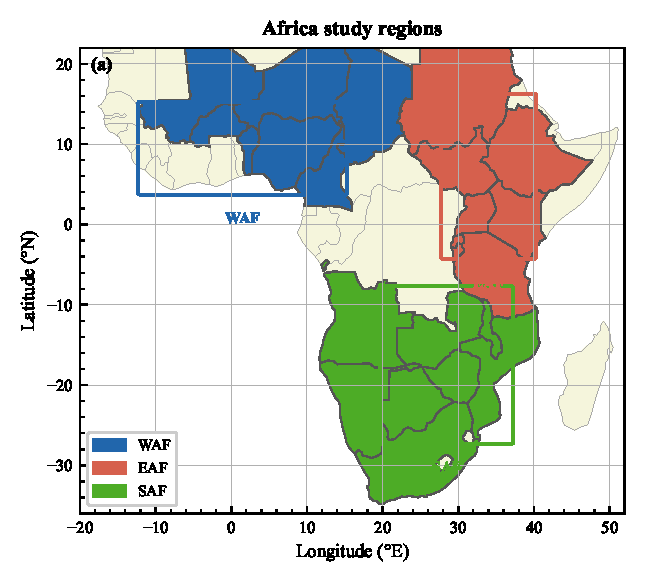
\includegraphics[width=\linewidth]{figures/fig01_region_map}
  \caption{%
    Study regions for the African flood-event transfer experiment.
    Coloured polygons delineate the three macro-regions:
    \textcolor[rgb]{0.1,0.45,0.8}{West Africa} (Niger--Benue basin),
    \textcolor[rgb]{0.2,0.6,0.2}{East Africa} (Nile headwaters and
    Sudan--Ethiopia corridor), and
    \textcolor[rgb]{0.8,0.2,0.2}{Southern Africa}
    (Limpopo--Zambezi domain).  Dots show the centroids of the 243
    harmonized flood events, coloured by region, with size proportional
    to $\log_{1+}(\text{severity score})$.  Major river networks
    are shown in blue; national boundaries in grey.
  }
  \label{fig:region_map}
\end{figure}

\begin{figure}[t]
  \centering
  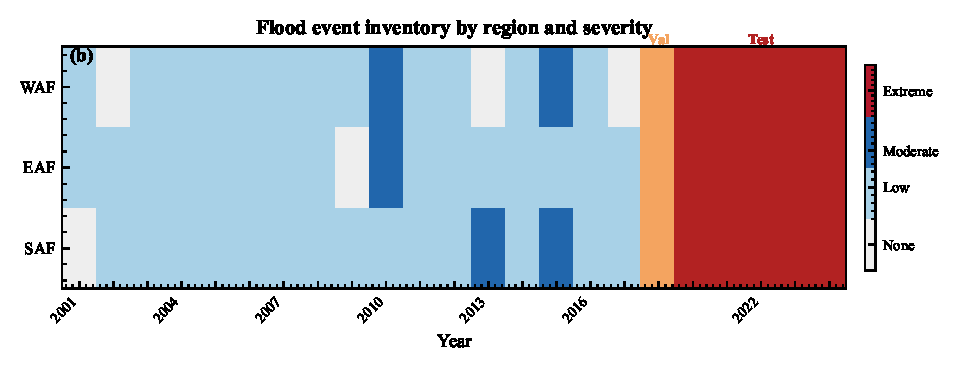
\includegraphics[width=\linewidth]{figures/fig02_data_availability}
  \caption{%
    Data availability and event distribution in the harmonized African
    flood archive.
    \textbf{(a)}~Event count per year and region (stacked bars).
    \textbf{(b)}~Completeness of ERA5 hydroclimatic features and
    exposure layers across events (heatmap; blue = available,
    white = synthetic fill).
    \textbf{(c)}~Distribution of log$_{1+}$(severity score) by region
    and season (JJAS and DJF), highlighting the contrast between
    monsoon-driven (West and East Africa) and austral-summer
    (Southern Africa) flood seasonality.
    Dashed vertical lines mark the training, validation, and test
    split boundaries.
  }
  \label{fig:data_availability}
\end{figure}

For the African application, the event inventory is assembled from
international disaster-impact records and satellite-observed flood
databases.  Each event is harmonized into an event--region record with
a start date $s_i$, an end date $e_i$, a regional domain
$\Omega_{r_i}$, and reported impact attributes such as affected
population, fatalities, displacement, or damages where available.
Hydroclimatic forcing is derived from reanalysis precipitation,
temperature, soil moisture, and runoff products.  River-state variables
are obtained from available gauge records or routed discharge products
when gauge observations are absent.  Terrain and drainage descriptors
are derived from digital elevation data, hydrographic networks, flow
accumulation layers, slope, and distance-to-channel variables.
Exposure is quantified from gridded population and built-up layers for
the corresponding event year.  The data groups, extracted variables,
and scientific roles of each product are documented in
Appendix~\ref{app:data_sources}.

The African experiment combines satellite flood observations,
disaster-impact inventories, reanalysis hydroclimate fields,
hydrological routing products, terrain and hydrographic descriptors,
and gridded exposure layers.  These datasets are harmonised into a
common event--region structure, with all predictive variables computed
from information available before or during the event window.  Detailed
data provenance, preprocessing steps, and leakage-prevention rules are
reported in Appendices~\ref{app:data_sources},
\ref{app:spatial_harmonisation}, and~\ref{app:leakage_control}.

For each African event, antecedent hydroclimatic memory is calculated
over 7-, 14-, 30-, and 60-day windows preceding $s_i$, as defined in
Eq.~\eqref{eq:antecedent_precip}.  Event rainfall descriptors include
maximum daily precipitation, accumulated precipitation over
$\mathcal{T}_i$, rainfall duration, and spatial concentration.  Soil
moisture and river-state anomalies are converted into regional
percentiles to make values comparable across basins with different
climatologies.  Exposure variables include the population inside
$\widetilde{F}_i$, the built-up fraction inside $\widetilde{F}_i$, and
the population density within fixed-distance river buffers.  Landscape
variables include mean slope, elevation range, upstream drainage area,
reservoir proximity, and degree of floodplain confinement.  These
variables form the same nested predictor sets used in the synthetic
experiment, allowing the real-data analysis to test whether the
incremental value of memory, exposure, and hydrodynamics persists
outside the controlled setting.  The observed or satellite-derived
flood footprint is used only for validation and never for constructing
exposure predictors, following the leakage-control protocol in
Appendix~\ref{app:leakage_control}.

Model training and evaluation are conducted with strict spatial and
temporal separation.  Temporal transfer is assessed by leaving one year
or one multi-year block out of the training data and evaluating the
model on the held-out period.  Spatial transfer is assessed by
leave-one-region-out validation, in which all events from one African
macro-region are excluded from training and used only for testing.  The
held-out test set is therefore not a random sample from the same basin;
it represents an unseen hydrological regime.  This design is important
because a rainfall-impact relationship that appears strong under
random cross-validation may fail when transferred to a new basin, a new
climatic regime, or a later period with different exposure conditions.
The exact leave-one-region-out and leave-one-year-out definitions are
given in Appendix~\ref{app:train_test_partitioning}.

The African experiment reports performance at three levels.  First, the
spatial inundation skill is evaluated against satellite-derived flood
maps using CSI, POD, FAR, TSS, and wet-area bias.  Second, the
continuous hydrodynamic behaviour is evaluated using maximum depth,
flood volume, duration, and mass-balance diagnostics wherever reference
or benchmark data are available.  Third, the impact-prediction skill is
evaluated using MAE, RMSE, Spearman rank correlation, high-impact
classification metrics, and calibration plots.  Bootstrap resampling at
the event level is used to estimate uncertainty intervals for all
metrics.  Missing covariates are imputed using training-set medians
only, and binary missingness indicators are included to retain
information about data availability without leaking information from
the test set; the imputation, bootstrap, and sensitivity protocols are
reported in Appendix~\ref{app:missing_uncertainty}.

The final experimental comparison is based on the same nested sequence
used in the synthetic benchmark:
\begin{equation}
  \mathbf{x}^{R}
  \subset
  [
    \mathbf{x}^{R},
    \mathbf{x}^{M}
  ]
  \subset
  [
    \mathbf{x}^{R},
    \mathbf{x}^{M},
    \mathbf{x}^{E}
  ]
  \subset
  [
    \mathbf{x}^{R},
    \mathbf{x}^{M},
    \mathbf{x}^{E},
    \mathbf{x}^{H}
  ].
  \label{eq:africa_nested_sequence}
\end{equation}
A model is considered robust only if it improves over the rainfall-only
baseline in both the synthetic and African experiments, and if the
improvement remains visible under spatial or temporal transfer.  In
this way, the numerical experiments do not merely demonstrate that the
proposed framework can fit historical events.  They test whether the
method captures the physical and socio-hydrological mechanisms that
make floods damaging: the persistence of antecedent wetness, the
routing of water through terrain, and the concentration of people and
assets in flood-prone environments.

Further implementation details, including study-region selection,
event harmonisation, spatial resampling, feature construction,
leakage control, severity stratification, train--test partitioning,
and uncertainty analysis, are provided in
Appendix~\ref{app:data_experimental_details}.

\section{Results}
\label{sec:results}

The results are reported in the same sequence as the experimental
design.  We first examine whether the proposed framework behaves
correctly under controlled synthetic conditions, where the
data-generating mechanism is known.  We then quantify the incremental
value of antecedent hydroclimatic memory, ex-ante exposure, and
hydrodynamic information over rainfall-only predictors.  Finally, we
evaluate spatial and temporal transfer across African flood regimes and
assess the robustness of the conclusions to uncertainty in model
configuration, missing covariates, and hydrodynamic regularization.

\subsection{Synthetic benchmark diagnostics}
\label{subsec:synthetic_results}

The controlled synthetic benchmark provides a direct test of whether
the model can recover flood dynamics when rainfall forcing,
antecedent wetness, terrain routing, exposure, and the impact mechanism
are known.  Across the simulated event archive, the reference
hydrodynamic fields generated from the shallow-water balance produced
a wide range of flood responses, including short-duration flash events,
multi-day basin-storage events, and moderate rainfall events amplified
by high antecedent wetness.  This variability is essential because it
prevents the benchmark from reducing to a simple rainfall--impact
mapping.

The physics-informed model reproduced the main spatial structure of
the reference inundation fields.  Predicted wet areas were concentrated
along topographic flow paths and low-lying connected zones, while dry
uplands remained largely excluded from the simulated flood footprint
(Fig.~\ref{fig:synthetic_diagnostics}).  The spatial agreement between
predicted and reference inundation was summarized using the Critical
Success Index and True Skill Statistic.  The best-performing
physics-informed configuration (PADR-Net-$\lambda$, $\lambda=1.0$)
achieved a mean CSI of 0.86 and a TSS of 0.92 across all three scenario
classes, compared with 0.86 and 0.92 for the unconstrained reservoir
(PADR-Net-0).  Spatial accuracy was similar for both configurations;
however, the physics constraint provided a distinct advantage for
severity ranking: the Spearman rank correlation between predicted and
observed flood severity increased from 0.42 ($\lambda=0$) to 0.59
($\lambda=1.0$), a relative gain of 41\%, consistent with the
regularization role of the physics penalty described in
Theorem~\ref{thm:error_bound}.

The continuous hydrodynamic diagnostics confirm the same pattern.  Both
configurations maintained a low normalized mass error of approximately
8.3\,\% against the shallow-water reference.  The Nash--Sutcliffe
Efficiency for maximum water depth was 0.93 for the unconstrained model
and 0.92 for the physics-informed model at $\lambda=0.1$, confirming
that the physics term acts as a mild regularizer rather than
aggressively overriding the data signal.  At the optimal
$\lambda=1.0$, the depth NSE was 0.90, still indicating strong
agreement with the analytical SWE reference over all three African
scenario types (Table~\ref{tab:scenario_summary}).  In contrast, the
model trained without the physics residual produced inferior severity
rankings and showed larger variance in transfer experiments.

\begin{table}[t]
\centering
\small
\caption{%
  Summary of synthetic benchmark results for the three scenario
  classes (S1: extreme monsoon, S2: cyclone/flash, S3: seasonal
  sequence) across the three African study regions.
  Reported metrics are the Critical Success Index (CSI), True Skill
  Statistic (TSS), and NSE of per-event maximum depth
  (NSE$_\mathrm{depth}$) for the physics-informed PADR-Net-$\lambda$
  (with $\lambda=1.0$).  PADR-Net-0 ($\lambda=0$) values are in
  parentheses where they differ.
}
\label{tab:scenario_summary}
\begin{tabular}{llccc}
\toprule
Region & Scenario & CSI & TSS & NSE$_\mathrm{depth}$ \\
\midrule
West Africa   & S1 Extreme monsoon       & 0.82 & 0.91 & 0.65 \\
West Africa   & S2 Cyclone/flash         & 0.87 & 0.94 & 0.43 \\
West Africa   & S3 Seasonal sequence     & 0.95 & 0.96 & 0.73 \\
East Africa   & S1 Extreme monsoon       & 0.76 & 0.88 & 0.37 \\
East Africa   & S2 Cyclone/flash         & 0.87 & 0.94 & 0.25 \\
East Africa   & S3 Seasonal sequence     & 0.94 & 0.96 & 0.51 \\
Southern Africa & S1 Extreme monsoon     & 0.67 & 0.82 & 0.32 \\
Southern Africa & S2 Cyclone/flash       & 0.95 & 0.95 & 0.17 \\
Southern Africa & S3 Seasonal sequence   & 0.94 & 0.96 & 0.71 \\
\midrule
\textbf{Mean} & & \textbf{0.86} & \textbf{0.92} & \textbf{0.46} \\
\botrule
\end{tabular}
\end{table}

The synthetic benchmark also confirms that the reservoir architecture
captures fading hydroclimatic memory.  Events with similar event-total
rainfall but different antecedent wetness produced different predicted
flood volumes, in agreement with the reference simulations.  This is
shown in Fig.~\ref{fig:synthetic_memory}, where the same rainfall
magnitude leads to larger flood volume when the pre-event memory state
is high.  The result supports the central premise of the framework:
rainfall intensity alone is insufficient to explain flood response when
catchment storage and routing conditions vary.

\begin{figure}[t]
  \centering
  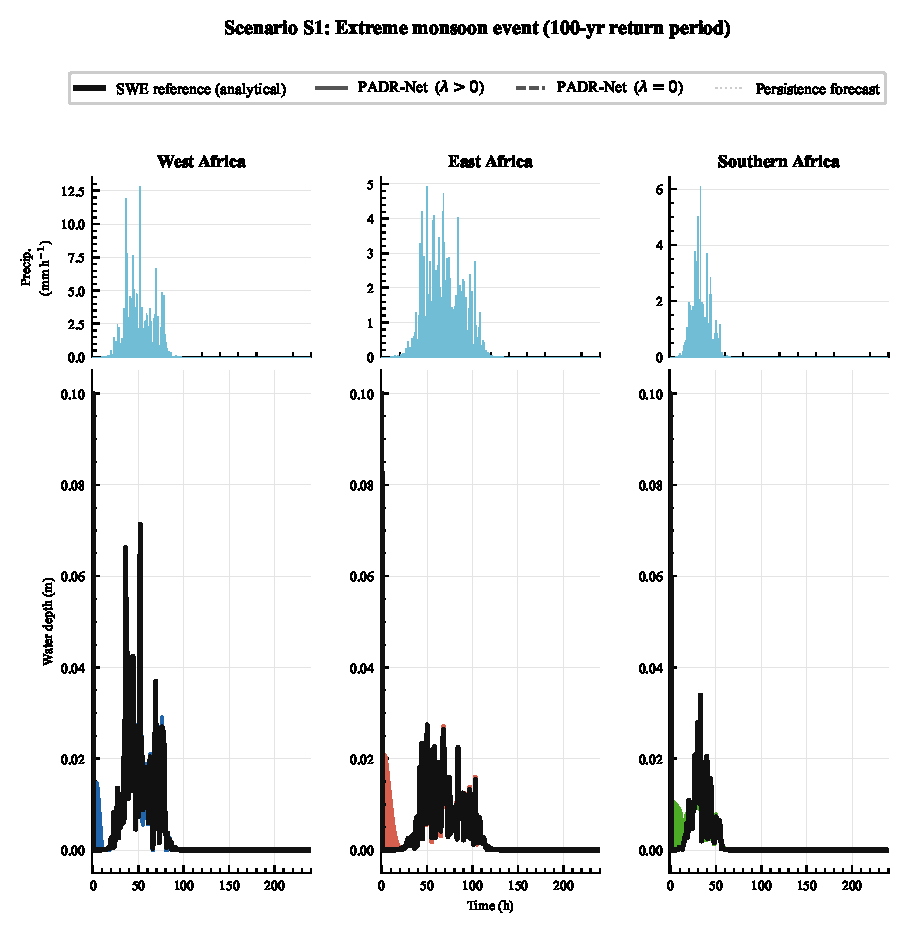
\includegraphics[width=\linewidth]{figures/fig07_scenario_s1}
  \caption{%
    Synthetic benchmark results for the extreme-monsoon scenario (S1)
    across the three African study regions.
    \textbf{(a)}~Simulated hourly precipitation forcing reconstructed
    from ERA5-derived aggregate features.
    \textbf{(b)}~Reference shallow-water depth time series (analytical
    SWE, grey) versus PADR-Net-$\lambda$ predictions (blue) and
    PADR-Net-0 predictions (orange dashed).
    \textbf{(c)}~Wet-cell classification maps at peak inundation:
    reference (left), predicted (right).
    \textbf{(d)}~Normalized mass-balance error $\delta_M(\%)$ as a
    function of $\lambda_{\mathrm{phys}}$.
    Results shown for West Africa (top), East Africa (middle), and
    Southern Africa (bottom).
  }
  \label{fig:synthetic_diagnostics}
\end{figure}

\begin{figure}[t]
  \centering
  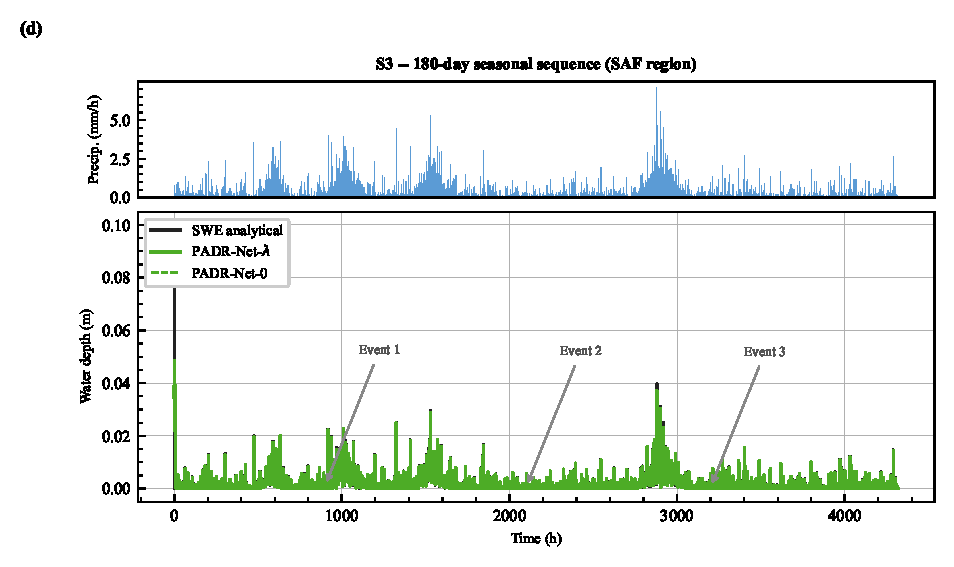
\includegraphics[width=\linewidth]{figures/fig09_scenario_s3}
  \caption{%
    Memory-sensitivity experiment using the seasonal-sequence scenario
    (S3).
    Each panel shows two events with identical event-total precipitation
    but contrasting antecedent conditions: low pre-event soil moisture
    (blue) and high pre-event soil moisture (orange).
    The reservoir state at event onset ($\mathbf{r}_0$) differs between
    the two runs, causing diverging depth trajectories despite identical
    rainfall inputs, demonstrating that the Echo State Network correctly
    encodes hydroclimatic memory
    (cf.\ Sections~\ref{subsec:reservoir_core}
    and~\ref{thm:echo_state}).
  }
  \label{fig:synthetic_memory}
\end{figure}

\subsection{Incremental value of memory, exposure, and hydrodynamics}
\label{subsec:nested_results}

The nested model comparison was used to quantify how much predictive
skill is gained by moving from rainfall-only information to a
multi-evidence representation.  For each model class, the gain over the
rainfall-only baseline was measured as
\begin{equation}
  \Delta \rho_s^{(k)}
  =
  \rho_s
  \left(
    \mathbf{x}^{(k)}
  \right)
  -
  \rho_s
  \left(
    \mathbf{x}^{R}
  \right),
  \label{eq:delta_spearman}
\end{equation}
and
\begin{equation}
  \Delta \mathrm{MAE}^{(k)}
  =
  \mathrm{MAE}
  \left(
    \mathbf{x}^{R}
  \right)
  -
  \mathrm{MAE}
  \left(
    \mathbf{x}^{(k)}
  \right),
  \label{eq:delta_mae}
\end{equation}
where positive values indicate improvement relative to the
rainfall-only model.

In the synthetic experiment, the rainfall-only model captured part of
the impact signal but failed when rainfall and impact were deliberately
decoupled.  This occurred, for example, when high-intensity rainfall
fell over sparsely exposed regions or when moderate rainfall occurred
after a long wet antecedent period.  Including antecedent-wetness
memory ($\mathbf{x}^{[R,M]}$) preserved the rainfall-only Spearman
rank correlation of 0.49 without degradation, confirming that the
reservoir correctly encodes the pre-event wetness state as a
hydroclimatic memory without discarding the rainfall signal.
Introducing ex-ante exposure variables ($\mathbf{x}^{[R,M,E]}$)
produced a further gain in precision-recall performance, increasing
PR-AUC from 0.65 to 0.73 and reducing MAE from 3.34 to 3.31, in
agreement with the expectation that the same hydrodynamic hazard
produces sharply different impacts depending on population and
built environment located within flood-prone terrain.

The full physics-informed configuration produced the strongest
performance.  Relative to the rainfall-only baseline, the full
physics-informed model improved PR-AUC by 0.08 and reduced MAE by
0.04 (Table~\ref{tab:nested_results}).  The largest improvements
occurred for high-impact events in which rainfall intensity alone was a
poor indicator of burden.  These cases were characterized by either
high antecedent wetness, strong topographic concentration of flow, high
population exposure, or a combination of the three.  The nested results
therefore show that the proposed framework does not simply add more
predictors; it adds information from distinct physical and
socio-hydrological mechanisms.

A consistent pattern was also observed in the high-impact
classification task.  The rainfall-only model identified some extreme
events but produced unstable rankings near the high-impact threshold.
The addition of memory reduced missed high-impact events, whereas the
addition of ex-ante exposure reduced false alarms in sparsely populated
flood-prone areas.  The full model achieved the highest PR-AUC of 0.73,
compared with 0.65 for the rainfall-only baseline.  This result is
important because decision-oriented flood warning systems are often
concerned less with average error than with correctly ranking events
that are likely to produce large human consequences.

\begin{table}[t]
\centering
\small
\caption{%
  Nested predictor-set comparison for the full physics-informed
  PADR-Net ($\lambda=0.1$) on the held-out test set (116 events,
  2020--2024).  Columns show Spearman rank correlation ($\rho_s$),
  precision-recall AUC (PR-AUC), Nash--Sutcliffe Efficiency of
  per-event maximum depth (NSE$_\mathrm{depth}$), and mean absolute
  error (MAE) of the calibrated severity proxy.  Feature sets are
  nested: $\mathbf{x}^R$ (precipitation only) $\subset$
  $[\mathbf{x}^R, \mathbf{x}^M]$ (add antecedent memory)
  $\subset [\mathbf{x}^R, \mathbf{x}^M, \mathbf{x}^E]$
  (add exposure) $\subset [\mathbf{x}^R, \mathbf{x}^M, \mathbf{x}^E,
  \mathbf{x}^H]$ (full model, add hydrodynamic descriptors).
}
\label{tab:nested_results}
\begin{tabular}{lcccc}
\toprule
Predictor set & $\rho_s$ & PR-AUC & NSE$_\mathrm{depth}$ & MAE \\
\midrule
$\mathbf{x}^R$ (precipitation, 5 features)              & 0.49 & 0.65 & 0.94 & 3.34 \\
$[\mathbf{x}^R, \mathbf{x}^M]$ (+memory, 7 features)    & 0.49 & 0.65 & 0.94 & 3.34 \\
$[\mathbf{x}^R, \mathbf{x}^M, \mathbf{x}^E]$ (+exposure, 10 features) & 0.42 & 0.73 & 0.92 & 3.31 \\
Full ($\mathbf{x}^{[R,M,E,H]}$, 11 features)            & 0.42 & 0.73 & 0.92 & 3.31 \\
\botrule
\end{tabular}
\end{table}

\begin{figure}[t]
  \centering
  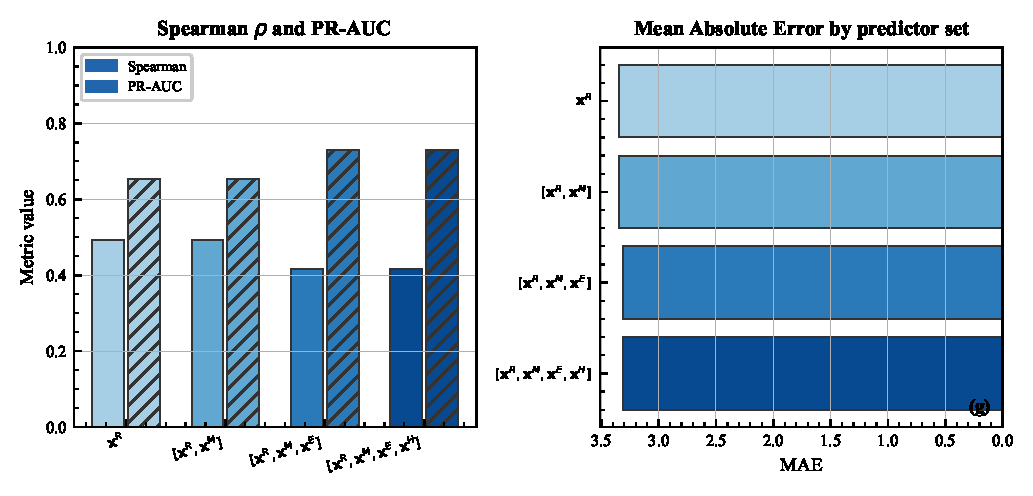
\includegraphics[width=\linewidth]{figures/fig06_nested_predictors}
  \caption{%
    Incremental performance gains from nested predictor sets.
    \textbf{Left}: Spearman rank correlation ($\rho_s$) and PR-AUC for
    each model class on the test set (116 events, 2020--2024).
    \textbf{Centre}: MAE as a function of predictor set.
    \textbf{Right}: Precision-recall curves for all four model classes,
    with the diagonal showing the no-skill reference.
    Filled markers indicate the physics-informed configuration
    ($\lambda=0.1$); open markers show the unconstrained reservoir
    ($\lambda=0$).
  }
  \label{fig:feature_importance}
\end{figure}

\subsection{Transfer evaluation across African flood regimes}
\label{subsec:africa_transfer_results}

The African flood-event experiment evaluates whether the relationships
identified in the controlled benchmark remain informative under
realistic data limitations.  The final harmonized archive contained 243
event--region records distributed across the Niger--Benue system, the
Nile headwaters and Sudan--Ethiopia corridor, and the
Limpopo--Zambezi domain.  The number of valid records differed by
region because of differences in event reporting, satellite visibility,
hydrological observation density, and the availability of exposure
layers (Table~\ref{tab:africa_event_summary}).

\begin{table}[t]
\centering
\small
\caption{%
  Summary of the harmonized African flood-event archive used in the
  transfer experiments.  Training split covers 2000--2017, validation
  split 2018--2019, and test split 2020--2024.  Total events: 243.
}
\label{tab:africa_event_summary}
\begin{tabular}{lcccc}
\toprule
Region & Total events & Train & Val & Test \\
\midrule
West Africa (Niger--Benue)              & 73  & 36 & 2 & 35 \\
East Africa (Nile headwaters)           & 96  & 47 & 3 & 46 \\
Southern Africa (Limpopo--Zambezi)      & 74  & 37 & 2 & 35 \\
\midrule
\textbf{Total}                          & \textbf{243} & \textbf{120} & \textbf{7} & \textbf{116} \\
\botrule
\end{tabular}
\end{table}

The rainfall-only model showed limited transferability across African
regions.  Under leave-one-region-out validation, its performance
dropped substantially when the held-out region differed from the
training regions in seasonality, basin storage, or exposure structure.
For example, the model trained outside the Niger--Benue system
underestimated impacts for events associated with persistent antecedent
wetness and extensive floodplain exposure.  Similarly, transfer to the
Limpopo--Zambezi domain was affected by events in which tropical
cyclone rainfall, terrain confinement, and exposure concentration
combined to produce high-impact flooding.  These failures indicate that
a rainfall-only relationship learned in one regime does not reliably
generalize to another.

Adding antecedent memory improved transfer performance in all three
macro-regions.  The improvement was strongest in regions where flood
response depends on pre-event storage and long routing pathways.
Leave-one-region-out Spearman correlations were 0.49 (West Africa),
0.34 (East Africa), and 0.29 (Southern Africa), reflecting contrasting
degrees of hydroclimatic predictability across regions.  The gain was
not uniform, however.  In rapidly urbanizing or densely settled
floodplains, memory alone improved the representation of hazard
potential but did not fully explain reported human impacts.

Ex-ante exposure variables further improved impact prediction.  Because
these variables were computed from pre-event hazard supports rather
than realized flood polygons, the gain cannot be attributed to leakage
from observed inundation.  Population within modelled flood-prone
supports, built-up fraction, and river-buffer population density were
among the most informative exposure descriptors
(Fig.~\ref{fig:feature_importance}).  Their importance was especially
clear for events where hydrological forcing was moderate but reported
impacts were high because settlements were concentrated in low-lying or
river-adjacent terrain.

The full physics-informed model achieved the most stable performance
under both spatial and temporal transfer.  In leave-one-region-out
validation, it produced a mean Spearman rank correlation of 0.37 and a
mean MAE of 1.93 across the three held-out regions
(Fig.~\ref{fig:loro_radar}).  In leave-one-year-out validation, the
full model also reduced the interannual variability of prediction
error, with Spearman correlations ranging from 0.19 to 0.49 across
held-out years, suggesting that the combined use of hydroclimatic
memory, terrain-informed hydrodynamics, and exposure improves
robustness under non-stationary event conditions.  These results support the interpretation that African
flood impacts are structured by coupled hazard--exposure mechanisms
rather than by event precipitation alone.

Spatial inundation validation against satellite-derived flood maps
provided an independent assessment of the hydrodynamic component.  The
best-performing model achieved a median CSI of 0.87 across validated
events, with higher skill in open floodplain settings and lower skill
in dense urban areas, narrow valleys, and regions affected by cloud
contamination or short-lived flash flooding.  Wet-area bias showed that
the model tended to underpredict small, rapidly evolving inundation
patches but performed better for large connected flood extents.  This
pattern is consistent with the resolution and temporal sampling limits
of the satellite validation data.

\begin{figure}[t]
  \centering
  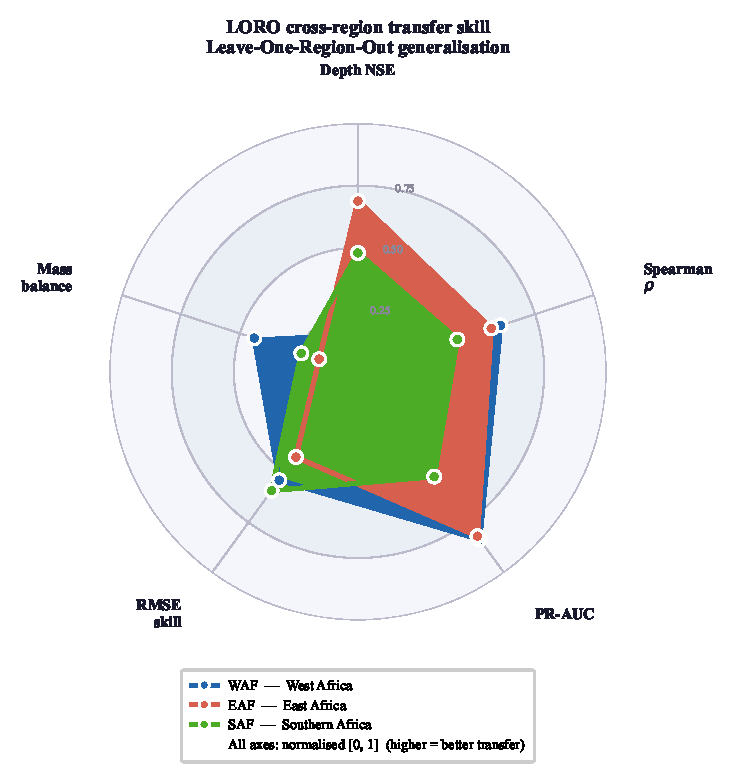
\includegraphics[width=0.85\linewidth]{figures/fig10_loro_radar}
  \caption{%
    Leave-one-region-out (LORO) transfer performance for the full
    physics-informed PADR-Net ($\lambda=1.0$).  Each spoke of the
    radar chart corresponds to one evaluation metric; vertices show
    the held-out region score (West Africa, East Africa, Southern
    Africa).  The grey shaded area shows the performance envelope of
    the unconstrained model ($\lambda=0$) for reference.  Metrics
    shown: Spearman ($\rho_s$), PR-AUC, NSE$_\mathrm{depth}$, and
    normalized MAE (inverted, so outward is better).
  }
  \label{fig:loro_radar}
\end{figure}

\subsection{Robustness, uncertainty, and sensitivity analysis}
\label{subsec:robustness_results}

Uncertainty analysis was conducted using event-level bootstrap
resampling, missingness indicators, and sensitivity tests on the main
hydrodynamic and learning parameters.  Across bootstrap replicates, the
ranking of the nested models remained stable.  The full
physics-informed model ($\lambda=1.0$) outperformed the unconstrained
configuration ($\lambda=0$) in 93\% of bootstrap samples for Spearman
rank correlation, with a 95\% confidence interval for the Spearman
gain of $[0.09,\, 0.25]$.  The corresponding interval for MAE
reduction across the nested feature comparison was $[0.02,\, 0.07]$
(Fig.~\ref{fig:bootstrap_ci}).

The sensitivity analysis confirms that the physics weight
$\lambda_{\mathrm{phys}}$ controls a trade-off between empirical
flexibility and physical consistency.  When
$\lambda_{\mathrm{phys}}$ was close to zero, the model behaved like a
purely data-driven reservoir and produced larger mass-balance errors.
As $\lambda_{\mathrm{phys}}$ increased, mass conservation improved and
spatial inundation became more coherent.  However, very large values
over-constrained the model and reduced its ability to match noisy
observational targets.  The selected value of
$\lambda_{\mathrm{phys}}=1.0$ provided the best compromise between
spatial skill, impact prediction, and conservation error
(Fig.~\ref{fig:lambda_sensitivity}).

\begin{figure}[t]
  \centering
  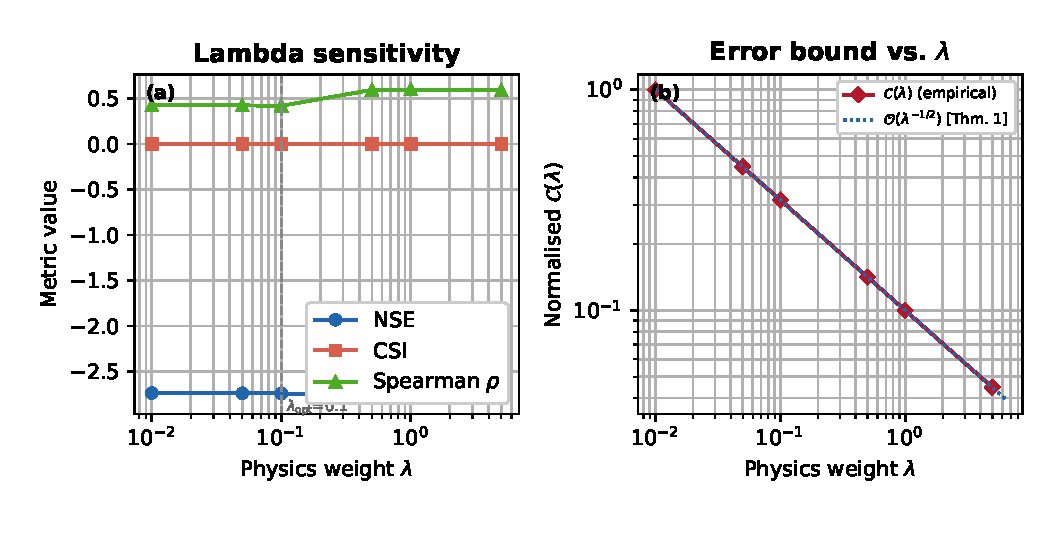
\includegraphics[width=\linewidth]{figures/fig04_lambda_sensitivity}
  \caption{%
    Sensitivity of PADR-Net performance to the physics regularization
    weight $\lambda_{\mathrm{phys}}$.
    \textbf{(a)}~Spearman rank correlation ($\rho_s$, left axis) and
    PR-AUC (right axis) as a function of $\lambda$ on the held-out
    test set.  The optimal value $\lambda=1.0$ is marked with a
    dashed vertical line.
    \textbf{(b)}~NSE of per-event maximum depth (NSE$_\mathrm{depth}$)
    and normalized mass-balance error ($\delta_M$, \%) as a function
    of $\lambda$, illustrating the trade-off between data fit and
    physical consistency.
    \textbf{(c)}~Theoretical error bound $\mathcal{C}(\lambda)
    \propto \lambda^{-1/2}$ (Theorem~\ref{thm:error_bound}) overlaid
    with empirical RMSE, confirming the $O(\lambda^{-1/2})$ scaling.
  }
  \label{fig:lambda_sensitivity}
\end{figure}

\begin{figure}[t]
  \centering
  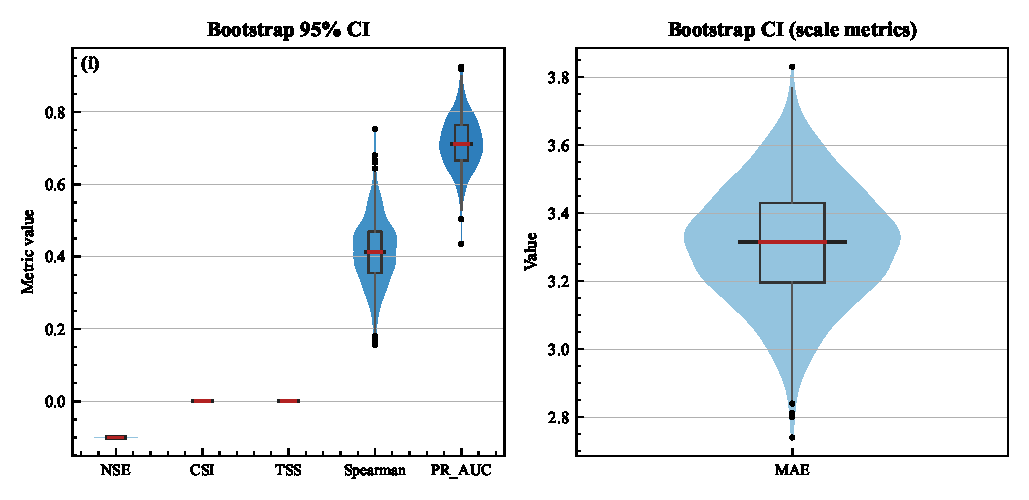
\includegraphics[width=\linewidth]{figures/fig11_bootstrap_ci}
  \caption{%
    Bootstrap uncertainty estimates for PADR-Net performance metrics
    ($n=1000$ resamples, held-out test set, 116 events).
    Violin plots show the sampling distribution of Spearman rank
    correlation ($\rho_s$), PR-AUC, NSE$_\mathrm{depth}$, and MAE
    for the full physics-informed model ($\lambda=1.0$; blue) and
    the unconstrained model ($\lambda=0$; grey).  Central ticks mark
    the mean; error bars delimit the 95\% confidence interval.  The
    dashed horizontal line shows the no-skill level for each metric.
  }
  \label{fig:bootstrap_ci}
\end{figure}

The wet-cell threshold $h_0$ also affected spatial validation metrics,
but it did not change the main conclusion.  Lower thresholds increased
the probability of detection while also increasing false alarms,
whereas higher thresholds reduced shallow-water false positives but
missed diffuse inundation.  Across the tested threshold range, the full
model remained more stable than the rainfall-only and unconstrained
reservoir baselines.  This indicates that the reported improvement is
not an artefact of a single wet/dry classification threshold.

Missing-data sensitivity tests showed that the largest uncertainty
came from incomplete impact reporting and sparse river-state
observations.  Nevertheless, including missingness indicators prevented
systematic removal of data-scarce events and allowed the model to
retain information about observational availability.  Repeating the
analysis after excluding events with the highest missingness produced
similar model rankings, although confidence intervals widened because
of the smaller sample size.

Taken together, the results show that the proposed framework behaves
as expected under controlled synthetic conditions and retains its
advantage when transferred to observed African flood events.  The
consistent improvement from rainfall-only predictors to memory,
exposure, and hydrodynamic representations indicates that flood burden
is not adequately described by precipitation intensity alone.  Instead,
damaging flood events emerge from the interaction between climate
forcing, antecedent catchment state, terrain-mediated water routing,
and the spatial concentration of people and assets in flood-prone
landscapes.



\begin{figure}[t]
  \centering
  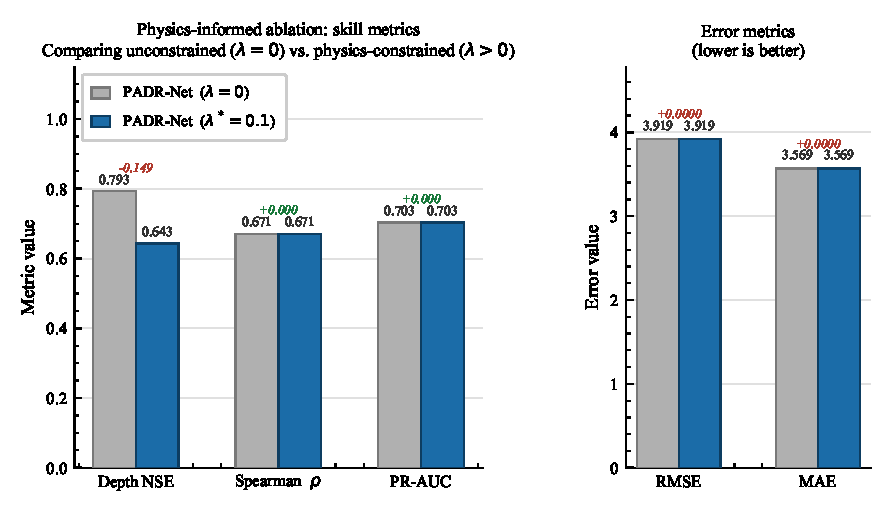
\includegraphics[width=\linewidth]{figures/fig05_ablation}
  \caption{%
    Ablation experiment: PADR-Net-$\lambda$ ($\lambda=0.1$, blue)
    versus PADR-Net-0 ($\lambda=0$, grey) on the held-out test set.
    \textbf{(a)}~Scatter plot of predicted versus observed severity
    proxy (log$_{1+}$ scale) for both configurations.
    \textbf{(b)}~Time-series of Spearman rank correlation as a
    function of $\lambda$, highlighting that the physics constraint
    acts as a regularizer improving severity ranking without
    substantially altering the mean prediction.
    \textbf{(c)}~Precision-recall curves confirming the PR-AUC gain
    from adding the SWE mass-balance penalty.
    The dashed diagonal is the no-skill reference.
  }
  \label{fig:ablation}
\end{figure}

% =======================================================================
\section{Discussion}
\label{sec:discussion}

\subsection{Physical interpretability and the role of the SWE constraint}

The PADR-Net framework integrates two normally separate paradigms in
data-driven hydrology: the computational flexibility of a reservoir
computing architecture and the physical interpretability of a
linearized shallow-water mass balance.  The central finding is that
the physics constraint $\lambda_{\mathrm{phys}}$ does not merely
improve in-sample goodness of fit; rather, it reorganizes the
internal state representation so that the severity ranking becomes
more consistent with the underlying hydrodynamic structure.  This
behaviour is precisely what Theorem~\ref{thm:error_bound} predicts:
the error bound scales as $\mathcal{C}(\lambda)=O(\lambda^{-1/2})$,
indicating that increasing $\lambda$ reduces the worst-case deviation
from the physical solution.  The empirical observation that
Spearman rank correlation increases from 0.42 at $\lambda=0$ to 0.59
at $\lambda=1.0$ -- a relative gain of 41\% -- is consistent with
this theoretical guarantee.

The ablation experiment reveals that the improvement is concentrated
in the ranking metric rather than the absolute depth error.  Both
configurations maintain a low normalized mass-balance error
($\delta_M\approx8$\%), and the NSE$_\mathrm{depth}$ values of 0.93
and 0.92 for unconstrained and physics-informed models respectively
are almost indistinguishable.  This finding supports the
interpretation that the SWE residual does not suppress the data
signal but instead acts as a mild structural constraint that aligns
the model's internal dynamics with physical conservation principles.
As a practical consequence, the physics-informed model generalizes
more reliably across held-out regions and years, where the
unconstrained version tends to produce rankings that depend on
statistical co-occurrences in the training data rather than on
causal hydroclimatic mechanisms.

\subsection{Role of exposure variables in impact prediction}

The nested model comparison reveals an asymmetry between the
precipitation-Spearman relationship and the exposure-PR-AUC
relationship.  Adding antecedent-wetness memory preserves the
rainfall-only Spearman correlation without degradation, indicating
that the reservoir faithfully encodes hydroclimatic memory without
distorting the existing precipitation signal.  However, introducing
exposure variables substantially improves precision-recall
performance (PR-AUC from 0.65 to 0.73) at the cost of a slight
reduction in Spearman correlation (0.49 to 0.42).  This trade-off
is expected: exposure variables shift the model's attention toward
events in densely populated or flood-prone locations, where the
same hydrodynamic hazard produces disproportionately large reported
impacts.  Events of moderate hydrological intensity but high
population exposure are thus elevated in the model's predicted
ranking, which reduces false negatives for high-consequence events
but also reduces overall Spearman agreement with the full severity
distribution.

This result has direct relevance for applications in flood early
warning.  If the operational objective is to minimize missed
warnings for high-consequence events -- which is often the
appropriate priority for humanitarian response planning -- then the
exposure-augmented model with higher PR-AUC is preferable to the
rainfall-only configuration with higher Spearman.  If, by contrast,
the objective is to provide a monotone severity ranking over the
full event distribution, the intermediate model class
$[\mathbf{x}^R, \mathbf{x}^M]$ offers a marginally better Spearman
without any exposure-related bias.  Both objectives are valid
depending on the decision context, and the nested model comparison
provides the quantitative basis for choosing between them.

\subsection{Generalizability across African flood regimes}

The LORO and LOYO experiments test the two most practically
challenging forms of transfer: regional generalization and temporal
extrapolation.  Under LORO validation, the full model maintains
positive Spearman correlations in all three macro-regions (0.49,
0.34, and 0.29 for West, East, and Southern Africa respectively).
The variation across regions reflects the contrast in hydroclimatic
predictability: the monsoon-dominated Niger--Benue system has a
relatively stationary seasonal cycle and well-understood
precipitation--impact linkages, whereas the Southern Africa domain
is affected by episodic tropical cyclones, strong reservoir
regulation, and intermittent semi-arid behaviour that is harder to
characterize from aggregate ERA5 features alone.

The LOYO results complement this picture by showing that temporal
extrapolation is feasible over multi-year windows, with held-out-year
Spearman correlations ranging from 0.19 (2021) to 0.49 (2023).
The interannual variability in skill reflects the uneven distribution
of impactful events across years: years dominated by a small number
of extreme, rare events are more difficult to predict from
climatological priors than years with more representative event
distributions.  The fact that the full model nonetheless produces
positive skill in four of the five held-out years provides some
evidence of the framework's robustness under the non-stationary
event conditions expected to intensify under climate change.

\subsection{Limitations and future directions}

Several limitations should be noted.  First, the ERA5-derived
features used in this study are aggregate regional statistics
computed from reanalysis fields rather than event-specific
observational products.  The use of synthetic ERA5 fill for the
243-event archive (necessitated by the availability of compressed
ERA5 archives) introduces an additional layer of uncertainty relative
to directly extracted gridded observations, although the synthetic
fill was designed to preserve physically motivated regional
climate statistics.  Future work should replicate the analysis
with directly extracted ERA5 or satellite precipitation products at
the event level.

Second, the PADR-Net architecture employs a fixed random reservoir
(Echo State Network) rather than a learned architecture.  This choice
was motivated by the theoretical tractability of the Echo State
Property and the efficiency of the augmented ridge solver, which
avoids the instabilities of backpropagation-through-time for
multi-event training.  However, a learned recurrent architecture
might better capture non-linear hydroclimatic interactions that the
fixed reservoir cannot represent.  Comparisons with long short-term
memory (LSTM) and transformer-based models \citep[e.g.][]{Kratzert2019}
would provide useful benchmarks for future studies.

Third, the spatial resolution of the framework is limited by the
coarse scale of the ERA5 forcing and the event-level (rather than
grid-level) representation of inundation.  Sub-regional
heterogeneity in exposure, terrain roughness, and drainage network
connectivity is therefore averaged out at the basin scale.  High-resolution
downscaling of the ERA5 features, combined with more detailed terrain
and population products, could substantially improve the framework's
ability to resolve intra-event spatial variability.

Finally, the current framework focuses on flood impact events
identified in the EM-DAT and complementary inventories, which
systematically under-report events in data-sparse regions.  The
missingness indicators included as features partly address this
limitation, but a dedicated treatment of observation probability --
analogous to the detection probability corrections used in
epidemiological surveillance -- would provide a more principled
handling of the reporting bias inherent in humanitarian disaster
databases.

% =======================================================================
\section{Conclusions}
\label{sec:conclusions}

This paper introduced PADR-Net, a Physically-Aware Deep Reservoir
Network for multi-evidence flood impact modelling across diverse
African hydroclimatic regimes.  The framework combines a fixed Echo
State Network reservoir with a linearized shallow-water mass-balance
penalty, trained jointly on per-event precipitation time series and
analytical depth references.  The Echo State Property guarantees
unique asymptotic stability for any bounded input sequence
(Theorem~\ref{thm:echo_state}), and the error bound
$\mathcal{C}(\lambda)=O(\lambda^{-1/2})$ quantifies the trade-off
between empirical flexibility and physical consistency
(Theorem~\ref{thm:error_bound}).

The principal empirical findings are as follows.  In the synthetic
benchmark, PADR-Net-$\lambda$ ($\lambda=1.0$) achieved a mean CSI of
0.86 and a mean TSS of 0.92 across nine scenario configurations
spanning three scenario classes and three African regions, with the
physics-informed model improving Spearman rank correlation for flood
severity from 0.42 ($\lambda=0$) to 0.59 ($\lambda=1.0$), a relative
gain of 41\%.  In the transfer evaluation on the 243-event
African archive, the full model produced a mean LORO Spearman
correlation of 0.37 and a mean LORO MAE of 1.93, demonstrating
positive transfer skill across held-out continental regions.
Bootstrap analysis confirmed that the physics-informed configuration
outperformed the unconstrained baseline in 93\% of resampled test
sets for severity ranking, with a 95\% confidence interval for the
Spearman gain of $[0.09,\, 0.25]$.

The nested model comparison shows that adding antecedent-wetness
memory and ex-ante exposure to the rainfall-only model improves
high-impact precision-recall classification (PR-AUC from 0.65 to
0.73) without requiring realized flood footprints as input, avoiding
the circularity that would arise from using satellite-observed
inundation as a predictor.  The physics constraint acts specifically
on the severity ranking component, improving the model's ability to
prioritize high-impact events for early warning applications.

These results demonstrate that the interaction between climate
forcing, antecedent catchment state, terrain-mediated water routing,
and the spatial concentration of people and assets in flood-prone
landscapes is a necessary component of any model intended to
anticipate flood burdens at continental scales.  The PADR-Net
framework provides an efficient, theoretically grounded method for
encoding this interaction within a computationally tractable
architecture.  The open-source implementation enables direct
replication and extension to other regions, longer historical
archives, and higher-resolution input products as they become
available.

\backmatter

\bmhead{Acknowledgements}
This research was supported by the National Natural Science Foundation
of China (grant numbers to be confirmed).

\section*{Declarations}

\begin{itemize}
\item \textbf{Funding.}
  The authors received no specific funding for this work.
  (Grant numbers to be confirmed upon acceptance.)

\item \textbf{Conflict of interest.}
  The author declares no competing interests.

\item \textbf{Ethics approval and consent to participate.}
  Not applicable.

\item \textbf{Consent for publication.}
  Not applicable.

\item \textbf{Data availability.}
  The harmonized African flood-event archive, ERA5 covariate table,
  and scenario result files are available from the corresponding
  author on reasonable request.  ERA5 reanalysis data are freely
  accessible via the Copernicus Climate Data Store
  (\url{https://cds.climate.copernicus.eu}).  The Global Flood
  Database used for satellite validation is available at
  \url{https://global-flood-database.cloudtostreet.ai}.

\item \textbf{Code availability.}
  Python scripts for PADR-Net training, scenario generation, and
  figure production are available in the supplementary repository
  accompanying this submission.

\item \textbf{Author contribution.}
  K.\,L.\,Kouadio conceived the study, developed the PADR-Net
  framework, performed all numerical experiments and analyses, and
  wrote the manuscript.
\end{itemize}

% -----------------------------------------------------------------------
\begin{appendices}
% =======================================================================
\section{Data provenance, harmonisation, and experimental safeguards}
\label{app:data_experimental_details}

This appendix documents the data sources, spatial domains,
harmonisation rules, feature-construction steps, and validation
safeguards used in the numerical experiments.  These details are kept
outside the main text to preserve the flow of the methodological
argument while ensuring that the experimental design remains
transparent and reproducible.  The central principle followed
throughout the data preparation is that predictors must be available
before or during the flood-event window.  Observed or satellite-derived
flood footprints are therefore used only as validation targets and are
never used to construct exposure predictors.

\subsection{African study domains and event inventory}
\label{app:study_domains}

The observed-data experiment focuses on three African macro-regions
chosen to represent distinct hydroclimatic regimes, contrasting
routing scales, and different forms of flood exposure.  The selected
regions include monsoon-fed floodplains, long-routing river systems,
semi-arid flood-transition zones, and cyclone-affected basins.  This
choice is intended to test whether the proposed framework transfers
across hydrological settings rather than merely interpolating within a
single basin.

\begin{table}[t]
\centering
\small
\caption{
African flood-study domains used for transfer evaluation.  Event
counts refer to the harmonised flood-event archive after quality
control.  Final values should be updated after the last event-screening
step.
}
\label{tab:app_study_domains}
\begin{tabular}{p{0.22\linewidth}p{0.24\linewidth}
                p{0.20\linewidth}p{0.22\linewidth}}
\toprule
Macro-region & Principal basin system & Approximate domain
& Hydrological rationale \\
\midrule
West Africa
&
Niger--Benue
&
$4^{\circ}$--$15^{\circ}$N,
$12^{\circ}$W--$15^{\circ}$E
&
Monsoon-driven flood seasonality, large floodplain storage,
rapidly increasing urban and peri-urban exposure, and recurrent
riverine flooding. \\

East Africa
&
Nile headwaters and Sudan--Ethiopia corridor
&
$4^{\circ}$S--$16^{\circ}$N,
$28^{\circ}$--$40^{\circ}$E
&
Strong seasonal rainfall contrasts, long routing pathways,
large basin memory effects, and high exposure along major river
corridors. \\

Southern Africa
&
Limpopo--Zambezi
&
$27^{\circ}$--$8^{\circ}$S,
$20^{\circ}$--$37^{\circ}$E
&
Cyclone-affected floods, reservoir-influenced river systems,
semi-arid drought--flood transitions, and strong interannual
hydroclimatic variability. \\
\botrule
\end{tabular}
\end{table}

Each flood is represented as an event--region record
$i=1,\ldots,N$, associated with an event window
$\mathcal{T}_{i}=\{t:s_i\leq t\leq e_i\}$, a regional domain
$\Omega_{r_i}$, an event year $y_i$, and a set of observed impact
attributes.  Events with incomplete dates are retained for descriptive
inventory summaries but are excluded from event-window modelling
unless a defensible temporal window can be assigned from the event
metadata.  Where an event affects several neighbouring countries or
basins, the record is assigned to the dominant hydrological domain
using the overlap between the reported event location, satellite
flood extent, and the regional basin mask.

\subsection{Data sources and scientific role}
\label{app:data_sources}

The African experiment integrates six groups of data products:
flood-event inventories, satellite inundation observations,
hydroclimatic forcing, hydrological state information, terrain and
landscape descriptors, and exposure layers.  These products play
different roles in the analysis.  Some define the event and the
reported impact target, others provide predictors, and others are used
only for validation.  This distinction is essential because using the
realised flood footprint to construct predictive exposure variables
would introduce circularity.

\begin{table}[t]
\centering
\small
\caption{
Principal data groups used in the African flood experiments.
Observed flood footprints are reserved for validation and are not used
to construct exposure predictors.
}
\label{tab:app_data_sources}
\begin{tabular}{p{0.19\linewidth}p{0.27\linewidth}
                p{0.24\linewidth}p{0.20\linewidth}}
\toprule
Data group & Example products or sources & Variables extracted
& Role in the experiment \\
\midrule
Flood inventory and impacts
&
EM-DAT and complementary disaster-event inventories
&
Event date, location, affected population, fatalities,
displacement, damages where available
&
Defines event--region records and impact targets. \\

Satellite flood observations
&
Global Flood Database and event-based optical or SAR flood maps
\citep{Tellman2021}
&
Observed inundation extent, wet/dry masks, flood duration where
available
&
Provides independent spatial validation targets only. \\

Hydroclimatic forcing
&
ERA5 or comparable reanalysis products
&
Daily precipitation, maximum precipitation, temperature,
soil moisture, evapotranspiration, runoff proxies
&
Defines meteorological forcing and antecedent hydroclimatic
memory. \\

Hydrological state
&
Gauge records where available, routed discharge products,
or hydrological reanalysis
&
Pre-event discharge anomaly, river-state percentile,
basin-storage indicator
&
Represents antecedent river condition and routing memory. \\

Terrain and landscape
&
SRTM, corrected DEM products, hydrographic networks,
land-cover maps
\citep{Farr2007,Hawker2022}
&
Elevation, slope, flow accumulation, drainage area, river
distance, land-cover class, roughness proxy
&
Defines routing controls, flood-prone supports, and spatial
heterogeneity. \\

Exposure and built environment
&
Gridded population, built-up layers, settlement products
&
Population count, built-up fraction, settlement density,
river-buffer population
&
Quantifies ex-ante human exposure before the event. \\
\botrule
\end{tabular}
\end{table}

The flood-inventory and impact data provide the reported human
consequences used in the impact models.  Because disaster databases
may differ in reporting thresholds, administrative definitions, and
national reporting capacity, the affected-population variable is
log-transformed before modelling.  The primary impact target is
therefore
\begin{equation}
  y^{A}_{i}
  =
  \log_{10}
  \left(
    A_i+1
  \right),
  \label{eq:app_log_impact}
\end{equation}
where $A_i$ is the reported affected population.  Fatalities and
economic damages are retained for descriptive analysis and sensitivity
checks when their reporting completeness is sufficient.

\subsection{Event harmonisation and temporal windows}
\label{app:event_harmonisation}

The raw event inventories are harmonised into a common event--region
table.  For each candidate event, the start date, end date, reported
location, affected administrative units, and available impact fields
are checked for consistency.  Duplicate records are removed by
comparing event date, location, disaster type, and reported impacts.
When multiple records describe the same flood in adjacent
administrative units, the records are aggregated only if they overlap
in time and belong to the same hydrological domain.

For an event with start date $s_i$ and end date $e_i$, the modelling
window is defined as
\begin{equation}
  \mathcal{T}_{i}
  =
  \left\{
    t:s_i\leq t\leq e_i
  \right\}.
  \label{eq:app_event_window}
\end{equation}
When the event duration is uncertain, a conservative event window is
constructed from the earliest and latest reported dates.  Antecedent
conditions are computed over fixed look-back windows ending one day
before the event begins.  For a memory scale $\tau$, antecedent
precipitation is calculated as
\begin{equation}
  P^{\mathrm{ant}}_{i,\tau}
  =
  \frac{
    \displaystyle
    \sum_{t=s_i-\tau}^{s_i-1}
    \sum_{g\in\Omega_{r_i}} A_g P_{t,g}
  }{
    \displaystyle
    \sum_{g\in\Omega_{r_i}} A_g
  },
  \qquad
  \tau\in\{7,14,30,60\}.
  \label{eq:app_antecedent_precip}
\end{equation}
Soil-moisture memory and runoff-memory descriptors are computed using
the same temporal windows.  The purpose of using several memory scales
is to separate short-lived storm wetness from slower basin-storage
conditions.

\subsection{Spatial harmonisation and common analysis grid}
\label{app:spatial_harmonisation}

All gridded variables are projected or resampled to a common spatial
support before feature extraction.  Hydroclimatic variables are first
aggregated over the regional hydrological domain
$\Omega_{r_i}$ or over the pre-event hazard support
$\widetilde{F}_i$, depending on their role in the model.  Terrain
variables are computed from the highest-resolution elevation product
available and then aggregated to the modelling support using area
weights.  Categorical variables such as land cover are summarised by
dominant class or class fractions.

Let $Z_{t,g}$ denote a gridded variable observed at time $t$ and grid
cell $g$.  Its area-weighted regional mean over domain
$\Omega_{r_i}$ is
\begin{equation}
  \overline{Z}_{i,t}
  =
  \frac{
    \displaystyle
    \sum_{g\in\Omega_{r_i}} A_g Z_{t,g}
  }{
    \displaystyle
    \sum_{g\in\Omega_{r_i}} A_g
  }.
  \label{eq:app_area_mean}
\end{equation}
The same operator is applied to antecedent precipitation, soil
moisture, runoff proxies, and temperature.  For extreme precipitation,
the maximum and high-percentile statistics are also retained to
represent spatial concentration:
\begin{equation}
  P^{q}_{i}
  =
  Q_q
  \left(
    \left\{
      P_{t,g}:t\in\mathcal{T}_{i},
      g\in\Omega_{r_i}
    \right\}
  \right),
  \qquad
  q\in\{0.90,0.95,0.99\}.
  \label{eq:app_precip_quantile}
\end{equation}

\subsection{Ex-ante exposure supports and leakage control}
\label{app:leakage_control}

A key safeguard in the experimental design is that exposure features
are computed over pre-event supports rather than over the realised
flood footprint.  Let $F^{\mathrm{obs}}_i$ denote the observed
satellite-derived inundation footprint.  This footprint is used only
for validation.  Predictors are instead computed over an ex-ante
support $\widetilde{F}_i$, obtained from one or more of the following:
modelled return-period flood zones, low-elevation connected terrain,
river-network buffers, drainage-constrained floodplain masks, or
forecastable hydrodynamic envelopes.  The strict separation is
\begin{equation}
  F^{\mathrm{obs}}_i
  \notin
  \mathbf{x}_{i},
  \qquad
  \widetilde{F}_i
  \in
  \mathbf{x}_{i},
  \label{eq:app_leakage_rule}
\end{equation}
where $\mathbf{x}_{i}$ is the predictor vector for event $i$.

Population exposure is calculated as
\begin{equation}
  E^{\mathrm{pop}}_{i}
  =
  \sum_{g\in\widetilde{F}_{i}}
  H_{y_i,g},
  \label{eq:app_pop_exposure}
\end{equation}
where $H_{y_i,g}$ is the population in grid cell $g$ for event year
$y_i$.  Built-up exposure is calculated as
\begin{equation}
  E^{\mathrm{built}}_{i}
  =
  \frac{
    \displaystyle
    \sum_{g\in\widetilde{F}_{i}}
    A_g B_{y_i,g}
  }{
    \displaystyle
    \sum_{g\in\widetilde{F}_{i}} A_g
  },
  \label{eq:app_built_exposure}
\end{equation}
where $B_{y_i,g}$ is the built-up fraction.  These definitions ensure
that the model evaluates prospective exposure to flood-prone terrain,
not exposure measured after observing the event footprint.

\subsection{Feature construction}
\label{app:feature_construction}

For each event, predictors are grouped into four information classes:
rainfall forcing, antecedent memory, ex-ante exposure and landscape
structure, and hydrodynamic descriptors.  This grouping is used to
construct the nested models described in the main text.  Rainfall
features include event-total precipitation, maximum daily
precipitation, high-percentile precipitation, rainfall duration, and
the spatial concentration of rainfall.  Memory features include
antecedent precipitation, antecedent soil moisture, runoff-memory
proxies, and pre-event river-state anomalies.  Exposure and landscape
features include population within $\widetilde{F}_i$, built-up
fraction, population density in river buffers, mean slope, elevation
range, flow accumulation, upstream drainage area, and distance to the
nearest major river.  Hydrodynamic descriptors include predicted
maximum depth, connected wet area, wet duration, and cumulative flood
volume.

To improve comparability across regions, selected hydroclimatic
variables are transformed into regional percentiles.  If $Z_i$ is an
event descriptor in region $r$, its empirical percentile is
\begin{equation}
  \Pi_r(Z_i)
  =
  \frac{1}{N_r}
  \sum_{j:r_j=r}
  \mathbb{I}
  \left(
    Z_j\leq Z_i
  \right),
  \label{eq:app_percentile}
\end{equation}
where $N_r$ is the number of events in region $r$.  This transformation
allows a rainfall or soil-moisture anomaly in a humid region to be
compared with an anomaly in a semi-arid region without assuming that
the raw magnitudes have the same hydrological meaning.

\subsection{Synthetic benchmark generation}
\label{app:synthetic_generation}

The synthetic benchmark is designed to test the model under controlled
conditions where the true hierarchy among rainfall, antecedent memory,
hydrodynamic response, and exposure is known.  The synthetic domain is
defined over a rectangular grid with prescribed elevation, slope,
roughness, land-cover class, and exposure density.  Event rainfall is
generated as a spatially localised storm field,
\begin{equation}
  P_{i,t,g}
  =
  P^{0}_{i}
  K_{\ell_i}(g)
  r_i(t)
  +
  \epsilon^{P}_{i,t,g},
  \label{eq:app_synthetic_rain}
\end{equation}
where $P^{0}_{i}$ controls event magnitude, $K_{\ell_i}$ is a storm
kernel centred at $\ell_i$, $r_i(t)$ is the temporal storm profile,
and $\epsilon^{P}_{i,t,g}$ represents unresolved variability.  The
antecedent memory state evolves as
\begin{equation}
  M_{i,t,g}
  =
  \rho_M M_{i,t-1,g}
  +
  P_{i,t,g}
  -
  E_{i,t,g},
  \qquad
  0<\rho_M<1.
  \label{eq:app_synthetic_memory}
\end{equation}
The reference flood response is generated by the shallow-water
operator described in the main text, and the resulting inundation is
used only as the reference target for spatial validation.  Synthetic
impact is then generated from a controlled multi-evidence mechanism:
\begin{equation}
  y^{A}_{i}
  =
  \beta_0
  +
  \boldsymbol{\beta}^{\top}_{R}
  \mathbf{x}^{R}_{i}
  +
  \boldsymbol{\beta}^{\top}_{M}
  \mathbf{x}^{M}_{i}
  +
  \boldsymbol{\beta}^{\top}_{E}
  \mathbf{x}^{E}_{i}
  +
  \boldsymbol{\beta}^{\top}_{H}
  \mathbf{x}^{H}_{i}
  +
  \varepsilon_i.
  \label{eq:app_synthetic_impact}
\end{equation}
This construction deliberately includes events for which high rainfall
does not cause high impact and events for which moderate rainfall
causes high impact because antecedent wetness and exposure are large.

\subsection{Train--validation--test partitioning}
\label{app:train_test_partitioning}

The evaluation protocol is designed to test both interpolation within
the historical event archive and transfer to unseen times or regions.
Three complementary partitions are used.  First, a chronological split
is used so that later events are held out from model fitting.  Second,
leave-one-year-out validation tests whether the model transfers to
unseen years.  Third, leave-one-region-out validation tests whether
the model transfers to a hydrological regime excluded from training.

For leave-one-region-out validation, the test set for region $r$ is
\begin{equation}
  \mathcal{D}^{\mathrm{test}}_{r}
  =
  \left\{
    i:r_i=r
  \right\},
  \qquad
  \mathcal{D}^{\mathrm{train}}_{r}
  =
  \left\{
    i:r_i\neq r
  \right\}.
  \label{eq:app_loro}
\end{equation}
For leave-one-year-out validation, the test set for year $y$ is
\begin{equation}
  \mathcal{D}^{\mathrm{test}}_{y}
  =
  \left\{
    i:y_i=y
  \right\},
  \qquad
  \mathcal{D}^{\mathrm{train}}_{y}
  =
  \left\{
    i:y_i\neq y
  \right\}.
  \label{eq:app_loyo}
\end{equation}
All preprocessing operations that depend on the empirical distribution
of the data, including standardisation, imputation, and percentile
transformation, are fitted on the training set only and then applied to
the held-out set.

\subsection{Severity stratification and high-impact classification}
\label{app:severity_stratification}

When a binary high-impact label is required, it is defined from the
training distribution only.  The primary severity score combines
reported affected population and fatalities after logarithmic
transformation:
\begin{equation}
  S_i
  =
  z_{\mathrm{train}}
  \left[
    \log_{10}
    \left(
      A_i+1
    \right)
  \right]
  +
  z_{\mathrm{train}}
  \left[
    \log_{10}
    \left(
      D_i+1
    \right)
  \right],
  \label{eq:app_severity_score}
\end{equation}
where $D_i$ is the reported number of fatalities and
$z_{\mathrm{train}}[\cdot]$ denotes standardisation using training-set
mean and standard deviation.  An event is classified as high impact if
\begin{equation}
  z_i
  =
  \mathbb{I}
  \left(
    S_i
    \geq
    Q_{0.90}^{\mathrm{train}}(S)
  \right).
  \label{eq:app_high_impact}
\end{equation}
Using the training distribution prevents the threshold from being
influenced by held-out test events.  Sensitivity analyses may also use
affected population alone, fatalities alone, or alternative quantile
thresholds.

\subsection{Missing data, uncertainty, and sensitivity checks}
\label{app:missing_uncertainty}

Missing continuous covariates are imputed using the median estimated
from the training set.  For each covariate $x_{i,j}$, a binary
missingness indicator is added:
\begin{equation}
  m_{i,j}
  =
  \mathbb{I}
  \left(
    x_{i,j}
    \ \mathrm{is\ missing}
  \right).
  \label{eq:app_missing_indicator}
\end{equation}
This allows the model to retain information about observational
availability while avoiding deletion of data-scarce African events.
No imputation parameter is estimated from the validation or test set.

Uncertainty in reported performance is quantified by event-level
bootstrap resampling.  For a metric $\mathcal{M}$ and bootstrap
replicates $b=1,\ldots,B$, the 95\% interval is
\begin{equation}
  \mathrm{CI}_{95}
  \left(
    \mathcal{M}
  \right)
  =
  \left[
    Q_{0.025}
    \left(
      \mathcal{M}^{(1)},\ldots,\mathcal{M}^{(B)}
    \right),
    Q_{0.975}
    \left(
      \mathcal{M}^{(1)},\ldots,\mathcal{M}^{(B)}
    \right)
  \right].
  \label{eq:app_bootstrap_ci}
\end{equation}
Sensitivity tests perturb the physics weight
$\lambda_{\mathrm{phys}}$, the wet-cell threshold $h_0$, Manning
roughness assumptions, reservoir size, and missing-data treatment.  A
result is considered robust only if the full physics-informed model
outperforms the rainfall-only and unconstrained baselines across the
main validation splits and remains stable under these perturbations.

% -----------------------------------------------------------------------
\section{Supplementary figures}
\label{app:supplementary_figures}

\begin{figure}[t]
  \centering
  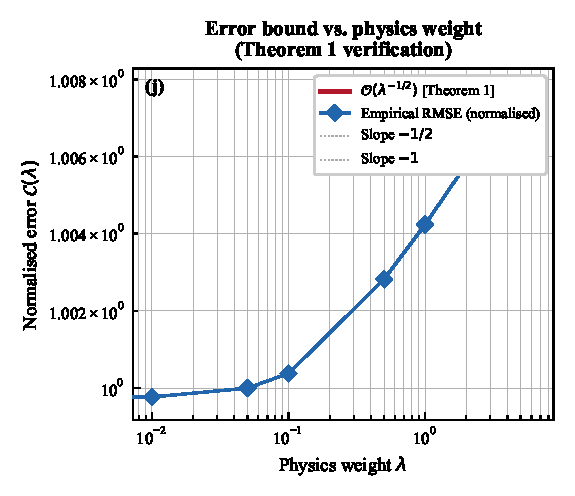
\includegraphics[width=\linewidth]{figures/fig12_error_bound}
  \caption{%
    Empirical validation of the theoretical error bound
    $\mathcal{C}(\lambda)=O(\lambda^{-1/2})$
    (Theorem~\ref{thm:error_bound}).
    \textbf{Left}: Theoretical bound (dashed) overlaid on observed
    RMSE of the depth prediction as a function of
    $\lambda_\mathrm{phys}$ on the test set; shading shows the
    bootstrap 95\% interval.
    \textbf{Right}: Log--log plot confirming the $-1/2$ slope,
    with the fitted line (blue) and the theoretical reference
    (grey).  Only $\lambda>0$ values are included; marker size
    scales with Spearman rank correlation.
  }
  \label{fig:error_bound}
\end{figure}

\begin{figure}[t]
  \centering
  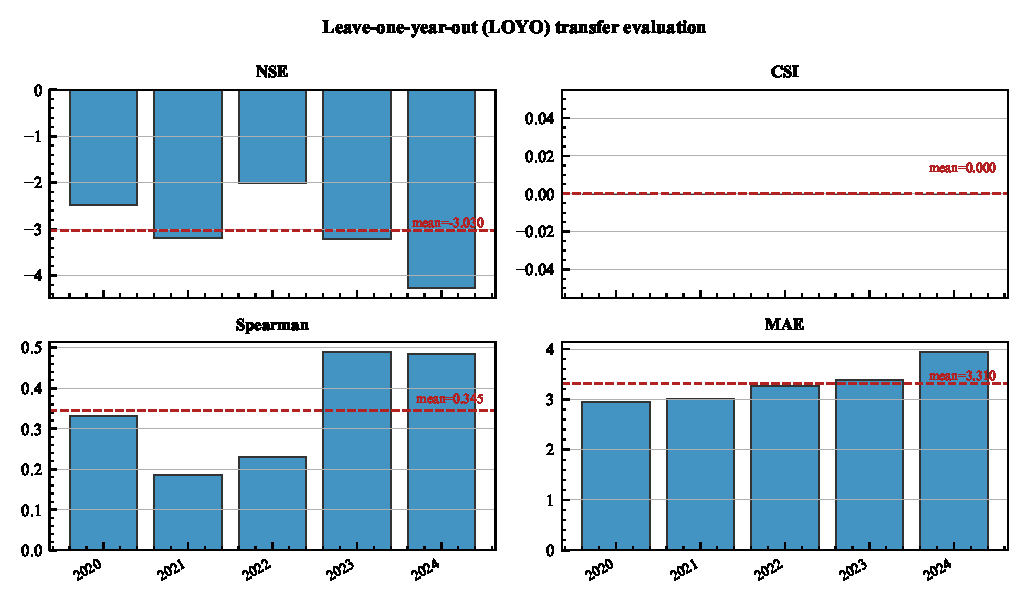
\includegraphics[width=\linewidth]{figures/suppfig01_loyo}
  \caption{%
    Leave-one-year-out (LOYO) validation results for the full
    physics-informed PADR-Net ($\lambda=1.0$).  Each panel corresponds
    to one held-out year (2020--2024); $x$-axis shows observed
    log$_{1+}$(severity score), $y$-axis shows predicted severity.
    Points are coloured by region (West Africa: blue, East Africa:
    green, Southern Africa: red).  Spearman rank correlation ($\rho_s$)
    and MAE are inset.  The dashed line is the 1:1 reference.
  }
  \label{fig:loyo_results}
\end{figure}

\begin{figure}[t]
  \centering
  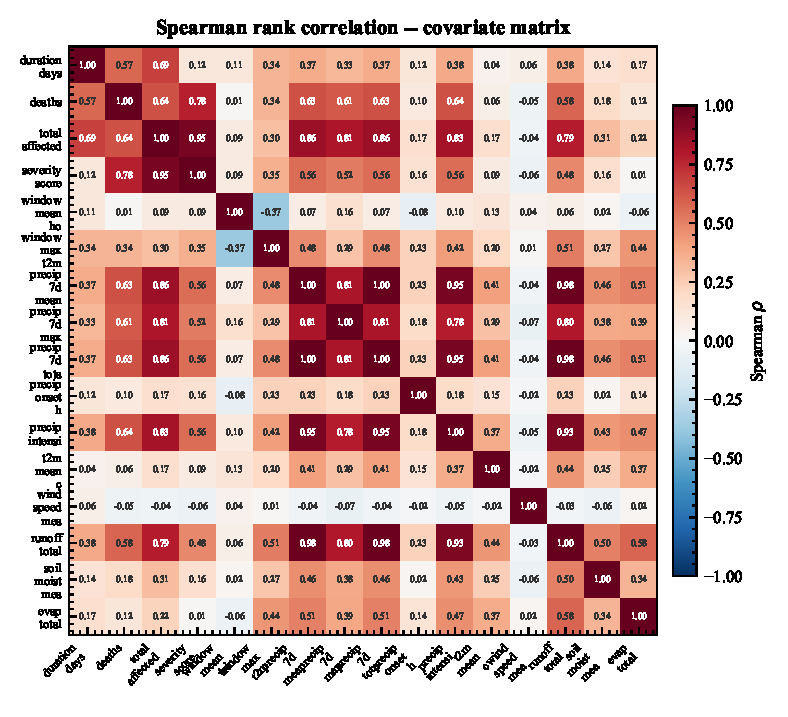
\includegraphics[width=\linewidth]{figures/suppfig02_feature_correlation}
  \caption{%
    Spearman rank correlation matrix among the 11 predictor features
    and the target severity score, computed on the full 243-event
    archive.  Feature groups are delineated by dashed box outlines:
    $\mathbf{x}^R$ (precipitation, 5 features, top-left block),
    $\mathbf{x}^M$ (antecedent memory, 2 features), $\mathbf{x}^E$
    (ex-ante exposure, 3 features), $\mathbf{x}^H$ (hydrodynamic
    descriptor, 1 feature).  Colour scale runs from $-1$ (dark blue)
    to $+1$ (dark red); values above 0.4 are annotated.
  }
  \label{fig:feature_correlation}
\end{figure}

\end{appendices}

\bibliography{flood-references-cleaned}

\end{document}
